%
%
% UCSD Doctoral Dissertation Template
% -----------------------------------
% https://github.com/ucsd-thesis/ucsd-thesis
%
%
% ----------------------------------------------------------------------
% WARNING: 
%
%   This template has not endorced by OGS or any other official entity.
%   The official formatting guide can be obtained from OGS.
%   It can be found on the web here:
%   http://grad.ucsd.edu/_files/academic-affairs/Dissertations_Theses_Formatting_Manual.pdf
%
%   No guaranty is made that this LaTeX class conforms to the official UCSD guidelines.
%   Make sure that you check the final document against the Formatting Manual.
%  
%   That being said, this class has been routinely used for successful 
%   publication of doctoral theses.  
%
%   The ucsd.cls class files are only valid for doctoral dissertations.
%
%
% ----------------------------------------------------------------------
% GETTING STARTED:
%
%   Lots of information can be found on the project wiki:
%   http://code.google.com/p/ucsd-thesis/wiki/GettingStarted
%
%
%   To make a pdf from this template use the command:
%     pdflatex template
%
%
%   To get started please read the comments in this template file 
%   and make changes as appropriate.
%
%   If you successfully submit a thesis with this package please let us
%   know.
%
%
% ----------------------------------------------------------------------
% KNOWN ISSUES:
%
%   Currently only the 12pt size conforms to the UCSD requirements.
%   The 10pt and 11pt options make the footnote fonts too small.
%
%
% ----------------------------------------------------------------------
% HELP/CONTACT:
%
%   If you need help try the ucsd-thesis google group:
%   http://groups.google.com/group/ucsd-thesis
%
%
% ----------------------------------------------------------------------
% BUGS:
%
%   Please report all bugs at:
%   https://github.com/ucsd-thesis/ucsd-thesis/issues
%
%
% ----------------------------------------------------------------------
% More control of the formatting of your thesis can be achieved through
% modifications of the included LaTeX class files:
%
%   * ucsd.cls    -- Class file
%   * uct10.clo   -- Configuration files for font sizes 10pt, 11pt, 12pt
%     uct11.clo                            
%     uct12.clo
%
% ----------------------------------------------------------------------



% Setup the documentclass 
% default options: 12pt, oneside, final
%
% fonts: 10pt, 11pt, 12pt -- are valid for UCSD dissertations.
% sides: oneside, twoside -- note that two-sided theses are not accepted 
%                            by OGS.
% mode: draft, final      -- draft mode switches to single spacing, 
%                            removes hyperlinks, and places a black box
%                            at every overfull hbox (check these before
%                            submission).
% chapterheads            -- Include this if you want your chapters to read:
%                              Chapter 1
%                              Title of Chapter
%
%                            instead of
%                              1 Title of Chapter
\documentclass[12pt,chapterheads]{ucsd}



% Include all packages you need here.  
% Some standard options are suggested below.
%
% See the project wiki for information on how to use 
% these packages. Other useful packages are also listed there.
%
%   http://code.google.com/p/ucsd-thesis/wiki/GettingStarted



%% AMS PACKAGES - Chances are you will want some or all 
%    of these if writing a dissertation that includes equations.
%  \usepackage{amsmath, amscd, amssymb, amsthm}

%% BONUS MATH
%  \usepackage{mathtools} 

%% MARGIN REQUIREMENTS IN TITLES - Hyphenation in a Section Title does not always respect margin settings in Latex.  To force no hyphentation, uncomment the package below.
%  \usepackage[raggedright]{titlesec} 

%% GRAPHICX - This is the standard package for 
%    including graphics for latex/pdflatex.
\usepackage{scrextend}
\usepackage{pslatex}
\usepackage{graphicx}
\usepackage{subcaption}
\usepackage{url}
\usepackage{xspace}

%% CAPTION
% This overrides some of the ugliness in ucsd.cls and
% allows the text to be double-spaced while letting figures,
% tables, and footnotes to be single-spaced--all OGS requirements.
% NOTE: Must appear after graphics and ams math
\makeatletter
\gdef\@ptsize{2}% 12pt documents
\let\@currsize\normalsize
\makeatother
\usepackage{setspace}
\doublespace
\usepackage[font=small, width=0.9\textwidth]{caption}
\usepackage[capposition=bottom]{floatrow} %force captions below figure per OGS requirement

%% SUBFIG - Use this to place multiple images in a
%    single figure.  Subfig will handle placement and
%    proper captioning (e.g. Figure 1.2(a))
% \usepackage{subfig}

%% TIMES FONT - replacements for Computer Modern
%%   This package will replace the default font with a
%%   Times-Roman font with math support.
% \usepackage[T1]{fontenc}
% \usepackage{mathptmx}

%% INDEX
%   Uncomment the following two lines to create an index: 
% \usepackage{makeidx}
% \makeindex
%   You will need to uncomment the \printindex line near the
%   bibliography to display the index.  Use the command
% \index{keyword} 
%   within the text to create an entry in the index for keyword.
%   To compile a LaTeX document with an index the 'makeindex'
%   command will need to be run.  See the wiki for more details.

%% HYPERLINKS
%   To create a PDF with hyperlinks, you need to include the hyperref package.
%   THIS HAS TO BE THE LAST PACKAGE INCLUDED!
%   Note that the options plainpages=false and pdfpagelabels exist
%   to fix indexing associated with having both (ii) and (2) as pages.
%   Also, all links must be black according to OGS.
%   See: http://www.tex.ac.uk/cgi-bin/texfaq2html?label=hyperdupdest
%   Note: This may not work correctly with all DVI viewers (i.e. Yap breaks).
%   NOTE: hyperref will NOT work in draft mode, as noted above.
% \usepackage[colorlinks=true, pdfstartview=FitV, 
%             linkcolor=black, citecolor=black, 
%             urlcolor=black, plainpages=false,
%             pdfpagelabels]{hyperref}
% \hypersetup{ pdfauthor = {Your Name Here}, 
%              pdftitle = {The Title of The Dissertation}, 
%              pdfkeywords = {Keywords for Searching}, 
%              pdfcreator = {pdfLaTeX with hyperref package}, 
%              pdfproducer = {pdfLaTeX} }
% \urlstyle{same}
% \usepackage{bookmark}


%% CITATIONS
% Sets citation format
% and fixes up citations madness
\usepackage{microtype}  % avoids citations that hang into the margin


%% FOOTNOTE-MAGIC
% Enables footnotes in tables, re-referencing the same footnote multiple times.
\usepackage{footnote}
\makesavenoteenv{tabular}
\makesavenoteenv{table}


%% TABLE FORMATTING MADNESS
% Enable all sorts of fun table tricks
\usepackage{rotating}  % Enables the sideways environment (NCPW)
\usepackage{array}  % Enables "m" tabular environment http://ctan.org/pkg/array
\usepackage{booktabs}  % Enables \toprule  http://ctan.org/pkg/array

\begin{document}

\definecolor{tealgreen}{rgb}{0.0, 0.51, 0.5}
\definecolor{cadmiumgreen}{rgb}{0.0, 0.42, 0.24}
\definecolor{darkolivegreen}{rgb}{0.33, 0.42, 0.18}

\newcommand{\stingw}[1]{{\color{tealgreen}[\textbf{\sc shuting}: \textit{#1}]}}
\newcommand{\TODO}[1]{{\color{blue}\textbf{\sc TODO}: \textit{#1}}}
\newcommand{\aurelia}[0]{\textsc{Aurelia}\xspace}

%% FRONT MATTER
%
%  All of the front matter.
%  This includes the title, degree, dedication, vita, abstract, etc..
%  Modify the file template_frontmatter.tex to change these pages.
%
%
% UCSD Doctoral Dissertation Template
% -----------------------------------
% http://ucsd-thesis.googlecode.com
%
%


%% REQUIRED FIELDS -- Replace with the values appropriate to you

% No symbols, formulas, superscripts, or Greek letters are allowed
% in your title.
\title{Accelerating Data Movement at Different Granularities in Datacenters}

\author{Shu-Ting Wang}
\degreeyear{\the\year}

% Master's Degree theses will NOT be formatted properly with this file.
\degreetitle{Doctor of Philosophy}

\field{Computer Science}
%\specialization{Anthropogeny}  % If you have a specialization, add it here

\chair{Professor Steven Swanson}
% Uncomment the next line iff you have a Co-Chair
% \cochair{Professor Cochair Semimaster}
%
% Or, uncomment the next line iff you have two equal Co-Chairs.
%\cochairs{Professor Chair Masterish}{Professor Chair Masterish}

%  The rest of the committee members  must be alphabetized by last name.
\othermembers{
Professor George C. Papen\\
Professor Geoffrey M. Voelker\\
Professor Jishen Zhao\\
}
\numberofmembers{4} % |chair| + |cochair| + |othermembers|


%% START THE FRONTMATTER
%
\begin{frontmatter}

%% TITLE PAGES
%
%  This command generates the title, copyright, and signature pages.
%
\makefrontmatter

%% DEDICATION
%
%  You have three choices here:
%    1. Use the ``dedication'' environment.
%       Put in the text you want, and everything will be formated for
%       you. You'll get a perfectly respectable dedication page.
%
%
%    2. Use the ``mydedication'' environment.  If you don't like the
%       formatting of option 1, use this environment and format things
%       however you wish.
%
%    3. If you don't want a dedication, it's not required.
%
%
\begin{dedication}
  To Olivia, my mom, and my late father
\end{dedication}


% \begin{mydedication} % You are responsible for formatting here.
%   \vspace{1in}
%   \begin{flushleft}
% 	To me.
%   \end{flushleft}
%
%   \vspace{2in}
%   \begin{center}
% 	And you.
%   \end{center}
%
%   \vspace{2in}
%   \begin{flushright}
% 	Which equals us.
%   \end{flushright}
% \end{mydedication}



%% EPIGRAPH
%
%  The same choices that applied to the dedication apply here.
%
% \begin{epigraph} % The style file will position the text for you.
%   \emph{A careful quotation\\
%   conveys brilliance.}\\
%   ---Smarty Pants
% \end{epigraph}

% \begin{myepigraph} % You position the text yourself.
%   \vfil
%   \begin{center}
%     {\bf Think! It ain't illegal yet.}
%
% 	\emph{---George Clinton}
%   \end{center}
% \end{myepigraph}


%% SETUP THE TABLE OF CONTENTS
%
\tableofcontents
\listoffigures  % Comment if you don't have any figures
\listoftables   % Comment if you don't have any tables



%% ACKNOWLEDGEMENTS
%
%  While technically optional, you probably have someone to thank.
%  Also, a paragraph acknowledging all coauthors and publishers (if
%  you have any) is required in the acknowledgements page and as the
%  last paragraph of text at the end of each respective chapter. See
%  the OGS Formatting Manual for more information.
%
\begin{acknowledgements}
%
I want to thank Olivia, my significant other and soon-to-be lifelong partner, for supporting me through my PhD journey.
%
It is a wild ride and thank you to be always on my side.

I want to thank all faculty members who invested their time mentoring me, 
%
Prof. George Porter for the first four years of advising that significantly shapes my taste and capability to do research, 
%
Prof. Steve Swanson for chairing my committee and giving me the last push to finish the dissertation,
%
Prof. Geoff Voelker for being on my committee and his wonderful operating system class,
%
Prof. George Papen for being on my committee and his insights on networking and optics, 
%
Prof. Alex Snoeren on all the critiques on my figures during weekly meetings, 
%
and Prof. Jishen Zhao for being willing to serve on my committee.

To Rajdeep, Yibo, Nishant, Stew, Audrey, Anil, Ariana, Alex, and all other tenants of room 3140, thanks for hanging out with me and being my friends.
%
The camaraderie is invaluable, and I will bear that in mind when I embark on my next journey.

To Rohan, Byung Hoon, and Amin, thanks for all the long talks and chats about research and the time of questioning of our life choices while still working on research. 

To Pierre-Louis, Weitao, and Dan, thanks for sharing my research interest on CXL and other topics.
%
I really enjoy all the online chats and meetings and the idea of I am not in this alone pushes me to finish the last chapter of this dissertation.

To Dr. Yiting Xia, Jialong, Yiming, and Federico, thanks for hosting me at MPI-INF in Saarbr\"{u}cken while I am working on this dissertation. 

To \textit{Fujimak}, \textit{SmallGGRen}, \textit{HakkaFish} and \textit{StanfordSneaky}, I really enjoy our time on Mario cart racing and chatting about lives and politics. I will keep your real names in private in case other people scoop you folks from me. 

I want to thank Yin Chin Foundation for their scholarship helping me for conference travel and supporting myself during finical instable times.

Coffee as the fuel for any research output is essential. I want to thank the great coffee shops and roasters in San Diego: Bird Rock coffee, the Art of Espresso, and Finjin. 

At last, I want to thank all my collaborators and co-authors, who are listed next.
%
Chapter~\ref{daronpon:chap}, in part, reprints material as it appears in a draft titled: 
"Daronpon: Datacenter-scale Sub-RTT Replica Selection for Low-latency Applications"
by Shu-Ting Wang, Stewart Grant, Keerthana Ganesan, George Porter, and Alex C. Snoeren.
%
The dissertation author was the primary researcher and author of this material.

Chapter~\ref{fianchetto:chap}, in part, reprints material as it appears in a paper titled: "Data Motion Acceleration: Chaining Cross-Domain Multi Accelerators"
by Shu-Ting Wang, Hanyang Xu, Amin Mamandipoor, Rohan Mahapatra, Byung Hoon Ahn, 
Soroush Ghodrati, Krishnan Kailas, Mohammad Alian, and Hadi Esmaeilzadeh~\cite{dmx:hpca:2024}.
% 
The dissertation author was the primary researcher and author of this material.

Chapter~\ref{aurelia:chap}, in part, reprints material as it appears in a published WORD'23 workshoppaper titled: 
"Aurelia: CXL Fabric with Tentacle" by Shu-Ting Wang and Weitao Wang~\cite{aurelia:words:2023}. 
%
The dissertation author was the primary researcher and author of this material.
%
\end{acknowledgements}


%% VITA
%
%  A brief vita is required in a doctoral thesis. See the OGS
%  Formatting Manual for more information.
%
\begin{vitapage}
\begin{vita}
  \item[2013] B.~S. in Computer Science, National Tsing Hua University, Taiwan
  \item[2015] M.~S. in Computer Science, National Tsing Hua University, Taiwan
  \item[2016] Information System Technician, Civil Service Training and Protection Commission, Taiwan 
  \item[2017] Research Assistant, National Taiwan University, Taiwan
  \item[2021] Hardware Systems Foundation Engineer Intern, Meta
  \item[2024] Visiting Ph.~D. student, Max Planck Institute for Informatics, Germany
  \item[2017-2024] Ph.~D. in Computer Science, University of California San Diego
\end{vita}
\begin{publications}
  \item Rohan Mahapatra, Soroush Ghodrati, Byung Hoon Ahn, Sean Kinzer, \textbf{Shu-Ting Wang}, Hanyang Xu,  Lavanya Karthikeyan, Hardik Sharma,  Amir Yazdanbakhsh,  Mohammad Alian, Hadi Esmaeilzadeh, “In-Storage Domain-Specific Acceleration for Serverless Computing” in Proceedings of the 29th ACM International Conference on Architectural Support for Programming Languages and Operating Systems, Volume 2 (ASPLOS), 2024
  %
  \item \textbf{Shu-Ting Wang}, Hanyang Xu, Amin Mamandipoor, Rohan Mahapatra, Byung Hoon Ahn, Soroush Ghodrati, Krishnan Kailas, Mohammad Alian, and Hadi Esmaeilzadeh, “Data Motion Acceleration: Chaining Cross-Domain Multi Accelerators” in Proceedings of 2024 IEEE International Symposium on High-Performance Computer Architecture (HPCA), 2024
  %
  \item \textbf{Shu-Ting Wang} and Weitao Wang, “Aurelia: CXL Fabric with Tentacle,” in Proceedings of the 4th Workshop on Resource Disaggregation and Serverless (WORDS), 2023
  %
  \item Rohan Mahapatra, Byung Hoon Ahn, \textbf{Shu-Ting Wang}, Hanyang Xu, and Hadi Esmaeilzadeh, “Exploring Efficient ML-based Scheduler for Microservices in Heterogeneous Clusters,” in Proceedings of 2022 MLArchSys Workshop, 2022
\end{publications}
\end{vitapage}


%% ABSTRACT
%
%  Doctoral dissertation abstracts should not exceed 350 words.
%   The abstract may continue to a second page if necessary.
%
\begin{abstract}
  The dissertation investigates redundant communication between servers for large-scale web and cache requests and redundant data movement between accelerators for compute-intensive applications. 
  %
  Redundancy is an impending and critical issue for data centers designed for hardware accelerators and disaggregated resources. 
  %
  The dissertation makes the following three contributions to address this. The first contribution of the dissertation is \daronpon. 
  %
  \daronpon dynamically load-balances and reroutes large-scale requests of web and cache applications on a microsecond timescale. 
  %
  \daronpon prevents these requests, stranded on busy servers with network congestion and long queuing delays, from being processed. Daronpon shows improvement in various service time characterizations of different applications.
  %
  The second contribution of the dissertation is \dmx. 
  %
  \dmx acts as a compute-enabled bypass for inter-accelerator communication. 
  %
  \dmx accelerates the data restructuring needed between accelerators and saves the data movement between accelerators and CPUs for compute-intensive applications.
  %
  \dmx shows improvement in a series of benchmarks involving different application domains.
  %
  The third contribution of the dissertation is \aurelia. 
  %
  \aurelia leverages the emerging interconnect of CXL to investigate the design of a scalable fabric for accelerators and fabric-attached memory expansion.
  %
  \aurelia improves routing and transport based on the current specification of CXL and shows performance improvement on machine learning and key-value store applications.
\end{abstract}


\end{frontmatter}






%% DISSERTATION

% A common strategy here is to include files for each of the chapters. I.e.,
% Place the chapters is separate files: 
%   chapter1.tex, chapter2.tex
% Then use the commands:
%   \include{chapter1}
%   \include{chapter2}
%
% Of course, if you prefer, you can just start with
%   \chapter{My First Chapter Name}
% and start typing away.

\chapter{Introduction}

\TODO{Make it fully 2-page with some rewriting and minor extension on details}
% Use Luiz André Barros' warehouse-scale computer arguments
Modern datacenters are warehouse-scale computers~\cite{datacenter-as-a-computer:2013}.
%
These warehouse-scale computers serve as the foundation of cloud computing, e.g. IaaS, SaaS, and serverless.
%
They host commodity servers equipped with many general-purposed CPU cores.
%
The servers are interconnected with 100 Gbps or faster network connections.
%
The servers are clustered into fleets for different functions. For example, some serve the web requests, some serve as data storage, and some serve as in-memory cache for frequently accessed objects.
%
Communication and data movement between servers are frequent and demonstrate diverse patterns depends on the mix of traffic from different functions \TODO{Cite Google, Meta and Azure's paper on workload and traces}.

Hardware accelerators are introduced to the datacenters given the rise of compute-intensive applications. 
%trend of deploying large machine learning models, 
%
These accelerators include Video codec, GPU, and TPU etc. deployed in the production datacenters nowadays. 
\TODO{cite TPU, VCU of Google and AWS inf/training hardware.}
% the increased footprint of non-CPU, accelerator hardware (GPU included as the general matrix accelerator and beyond).
% cloud datacenters are equipped with accelerators, ranging from generic GPUs, FPGAs, 
% to more workload-specific ASICs
%
The introduction of them demonstrates a move towards heterogeneous hardware landscape beyond a massive number of homogenous CPU cores.   
%
These accelerators accelerate specific compute-intensive workloads, such as video encoding and decoding, scientific computation, and large-scale machine learning.
%
% How do we connect hardware accelerators to the data movement?
They do not stand alone and operate on data moved from the host memory and return the results back to it. 
%
Thus, efficient data movement ensures that these dedicated accelerators are well-utilized.
%
In addition to the heterogeneous hardware landscape, resource disaggregation aims at efficient resource provision in the datacenters.
%  
Resource disaggregation allocates resources, such as CPU cores, memory capacity, and storage capacity, located on different physical machines in a logically unified manners~\cite{legoos:osdi:2018}
\TODO{Cite LegoOS and other 10 papers here. These citations should be already in the CXL paper}. 
%especially memory disaggregation.
%
The rationale behind disaggregation is to satisfy users with diverse requests on different resources \TODO{cite pond and other CXL papers}.
%
%\TODO{How do we connect disaggregation to increase data movement?}
Disaggregation, while aiming at efficient provision of resources, exposes the communication and data movement between CPU and memory/devices to a network fabric connecting the resources.   
%
The externalized communication and data movement that used to confined within a server stemming from disaggregation motivates the study of this thesis. 
%with the help of RDMA  and potentially CXL.

%A routable memory fabric connecting accelerators and disaggregated memory modules stands in the center of this issue and offers the benefit of 
%
%Redundant communication and data movement decreases the utilization of resources. Idled resources
%leave performance gain on the table.
%
%\stingw{the point of connections between accelerators and memory disaggregation is the memory fabric}
%
%\stingw{the large scale web/cache requests in datacenters can also be benefit from the memory disaggregation.}

%
The current datacenters demonstrate diverse communication and data movement patterns on different scale with their corresponding applications.
% 
We are, in particular, interested in the data movement of the following scenarios: 
(1) RPC communication for web and cache applications. The data movement is on the scale of a few packets to a few MBs in total size.
%
(2) Compute-intensive applications with the use of non cache-coherent accelerators. The data movement is with chunks of data on the scale up to 100s of MBs.
%
(3) Key-value store on disaggregated memory modules. The data movement operates on cacheline granularity to KBs in total size.  
%
In short, the current and conventional design of control and data plane shows redundant communication and data movement between servers for large scale web/cache requests and between accelerators for compute-intensive applications.
%
We argue that this redundancy is an impending and critical issue for datacenters designed for hardware accelerator and disaggregated resources. 
%
This thesis proposes to intelligently route the communication and data movement to bypass the congested or redundantly detoured path with a minimal addition of control logic. 
%
% The commonality shared by these seemingly different problems is that how we reason about 
% the communication/data movement pattern and provide systemic design and strategy for the problems.




%Data centers are the home of the cloud computing we know today.
%

\chapter{Background}
\TODO{We will do it later if the individual background paragraph look too scattered in terms of a good direction and flow for the entire thesis.}\\
\stingw{1. Datacenter basics, the idea of a rack, the idea of replicas, and the idea of load balancing}\\
\stingw{2. Accelerators, examples of them.}\\
\stingw{3. CXL background. This can be a lot of laundry listing but it can be very detailed to help us}
\chapter{Daronpon: Datacenter Load Balancing Across Racks}
\label{chap:daronpon}

%\def\checkmark{\tikz\fill[scale=0.4](0,.35) -- (.25,0) -- (1,.7) -- (.25,.15) -- cycle;}
\newcommand{\toolname}{Daronpon}
\newcommand{\systemname}{Daronpon}

\section{Introduction}
\label{sec:intro}

To improve both performance and fault tolerance, datacenter
applications are provisioned to scale horizontally, with replicated
instances frequently spread across multiple racks of servers.  These
replicas must be carefully managed to meet strict service-level
objectives (SLOs) for both throughput and
latency~\cite{killer_microseconds,tail_at_scale}. These requirements
have birthed an architectural paradigm of highly replicated
microservices that can (nearly) arbitrarily fan out to deliver
ever-higher throughput, and whose functionality is scoped to provide
microsecond-timescale responses with low latency even in the tail.

Realizing this design pattern in practice poses multiple engineering
challenges, however.  Microsecond-timescale services must be resilient
to low-level system and network perturbations and short-lived
congestion events to achieve consistent
performance~\cite{facebook_microburst}.  These events arise within the
operating system, runtime, and application software as well as due to
network-level incast events, where a large number of clients send to a
common destination server, causing in-network buffering and
substantial queuing delays~\cite{facebook_memcache}.  Moreover, the
potential impact of these so-called ``microbursts'' increases with
network bandwidth.  Large bursts can lead to packet drops and
necessitate end-to-end retransmissions.

Experience shows that a responsive and effective load-balancing
strategy is key to managing overall service latency.  Given the
ultra-low service times of many modern datacenter services, end-to-end
approaches driven by the clients and servers themselves are unlikely
to meet demands, as many component service (i.e., computation) times
are smaller than datacenter-wide network latencies. Instead, we focus
on in-network load balancing techniques carried out by network
switches or middle boxes---often generally referred to as
``dispatchers''.  Recent work has shown the benefits of load balancing
with a server rack, for example R2P2~\cite{r2p2} and
Racksched~\cite{racksched}.  These approaches take into account server
load balancing, building upon prior approaches to core scheduling in
individual servers~\cite{IX,shinjuku,shenango,seda}. Further,
Vargaftik et al.~\cite{lsq} show that, for the multiple-dispatcher
environments that we target, a stable and highly efficient load
balancing approach is possible through a carefully controlled exchange
of status updates between servers and dispatchers.

We present \toolname, an inter-rack load balancer targeted to network
services with sub-RTT service times.  \toolname\ periodically
exchanges service-load information between dispatchers, either through
explicit gossip messages or piggybacked onto redirected application
requests.  We employ a logarithmic thresholding approach to minimize
the network overhead of state-exchange messages while ensuring that
application requests are forwarded to replicas with good performance.
Our system decreases the 99th-percentile tail latency by up to a
factor of two over random replica selection across a variety of
application workloads, enables scaling across heterogeneous server
configurations, and provides performance gains for service times as
low as two microseconds.

\section{Background}
\label{sec:background}

%\textbf{Data Center Replication:}

Modern datacenter applications are
replicated~\cite{rocksdb,memcached,mongodb} to provide fault
tolerance, scalability and flexible response to load
fluctuations. Often, individual application components are replicated
on the order of three times for fault tolerance. In the case of
sharding for scalability, however, the number of replicas can be many
orders of magnitude higher and even grow
dynamically~\cite{facebook_shard,google_slicer,microsoft_service_fabric}
as needed to service demand.

\subsection{Datacenter load balancing}
%%
Traditional application or ``layer-4'' load balancers operate across
the set of back-end services and maintain connection consistency for
long-lived flows. They are generally implemented in software using
commodity servers~\cite{cheetah, maglev, beamer, ananta}, although
some have explored using switches with hardware support~\cite{duet,
  silkroad}.  While effective at responding to end-host-driven load
imbalances, they are ill-positioned to address transient
variations in service times.

Conversely, conventional layer-3 load-balancing techniques focus on
dispersing traffic load in the network, and do not address server
imbalance.  For example, equal-cost multi-path routing (ECMP) load
balances flows using a hash of their 5-tuple. ECMP is widely deployed
due to the benefits it gains from average-case statistical
multiplexing.  It is well known, however, to cause load imbalance due
to hash collisions and when links fail.  A variety of improvements to
ECMP have been proposed, many using the concept of
flowlets~\cite{conga, clove, HULA, letitflow}: a group of packets
within the same flow separated from others by a large enough time
interval. Other schemes load balance per
packet~\cite{drill,flowbender,hermes}. Each of these in-network
techniques are complementary to our work, as they load balance
exclusively based on the state of the network and not the end-host
applications.

\subsection{Microsecond timescales}

Despite practitioners' attempts to spread demand evenly across both
servers and network fabrics~\cite{facebook:sigcomm15}, a certain
degree of variability is inevitable.  Indeed, as links speeds of 100 and
400-Gbps become the norm, hosts and switches can experience
significant traffic bursts over short periods of time. These bursts,
while lasting only a few microseconds, can cause congestion, lead to
increased jitter, and result in packet
drops~\cite{facebook_microburst}. As a concrete example, a switch with
64~MB of packet memory will overflow in 1.9~ms at
100~Gbps~\cite{tofino2} under incast scenarios.  While these events
originate in the network, the effect of that queuing cascades at the
application. Congestion impacts performance directly as batches of
requests are delivered in very short time periods.  Existing
end-to-end techniques struggle to react to microbursts effectively as
the durations of the microbursts are shorter than the network RTT
which bounds the response time of any end-host approach.

%\emph{Rack-scale load balancing:}

\toolname\ targets microsecond-timescale services which
do not involve long-lived connections.
%Maintaining connections for
%microsecond timescale load balancing wastes precious resource on
%switches. \toolname\ is
(We support any request/response service on top of a connection-less
transport or one with migration ability~\cite{crab,quic}.)  Techniques
for dispatching such microsecond-duration requests within an end-host
operating system have been explored recently~\cite{IX, shinjuku, snap,
  shenango, zygos}.  These end-host-based approaches use load-aware
schedulers to direct requests to CPU cores and to quickly rebalance
those allocations.  Extensions to these techniques demonstrate similar
scheduling performance at the scope of a entire server
racks~\cite{r2p2, racksched}. These efforts make use of programmable
switches to track end-host load at the rate of millions of requests
per second~\cite{tofino2}. Both R2P2~\cite{r2p2} and
Racksched~\cite{racksched} are confined to services which operate
entirely within a single rack due to a single control point within the
ToR switch. This limits the applicability of these schemes for the
majority of replicated applications which are distributed throughout
the datacenter.

Researchers have also explored explicitly integrating different
replication techniques with programmable switching hardware to avoid
RTT delays, including chain replication~\cite{netchain},
Raft~\cite{hovercraft}, and Paxos~\cite{nopaxos}.  In-network
replication techniques have also been proposed to alleviate
read/write conflicts~\cite{harmonia} and
contention~\cite{pegasus}. \toolname\ operates under the assumption
that replicas are interchangeable for all requests; our
techniques could be extended to support distributed protocols, however
\toolname\ would require protocol specific information.

\section{Challenges}
\label{sec:challenges}

Theoretically, optimal load balancing is attainable with centralized
algorithms~\cite{jsq_fcfs} that maintain full knowledge of the global
instantaneous system load.  A proven-optimal algorithm,
join-the-shortest-queue (JSQ), ensures requests experience minimal
queuing delay.  Unfortunately, centralization prevents cross-rack
sharding and scale-out designs.  In contrast, fully decentralized
approaches (e.g. client-based power-of-two designs~\cite{power_of_2})
require network-wide message round trips to measure load. As the
service time of requests approaches that of an RTT, the cost of
probing increases the latency of the request and consumes more link
capacity (i.e two RTTs per request). Further, these approaches
struggle to react quickly to congestion given these long network-wide
round-trips. Load-balancing decisions made with information which has
aged by at least an RTT cannot react to microburst events which occur
on sub-RTT timescales.

\subsection{Microsecond load balancing at scale}

An ideal solution for microsecond load balancing at scale will therefore be
decentralized to avoid bottlenecks, designed to reduce probing overheads, and
designed to react nearly instantaneously to bursts.
Vargaftik et al.~\cite{lsq} demonstrated theoretically that distributed
load balancing for datacenter scale is possible. Their proposal, LSQ, has many
desirable properties such as a bounded measurement difference between true
server load and the load observed by a load balancer, which receives load
updates as messages using a variety of mechanisms~\cite{lsq}. 

We investigated via simulation an implementation of LSQ in which we
placed LSQ load balancers on core routers within a fat tree
network. Using core switches satisfies LSQ's theoretical assumptions
with regard to how each load balancer sees sever load by forcing all
packets through the core of the network to ensure that every request
is visible.  In this core-switch realization of LSQ, we find some
practical limitations.  The first of which is its (lack of) response
to microbursts. When requests target the same server, the available
bandwidth on the egress port of that server's associated top-of-rack
(ToR) switch is stressed, leading to drops~\cite{facebook_microburst}. These bursts
occur due to lack of coordination between core routers; they can be
prevented by making load-balancing decisions at the ToR instead.
%rather than at the core.

Hence, we propose to load balance on leaf ToRs directly. This
alteration has a variety of implications on LSQ's theoretical
approach. First, LSQ has approximate knowledge of all server
queues. By moving our load balancer to ToRs we lose instantaneous
knowledge of remote queues but gain up-to-date load information for
all of the servers in the rack beneath a ToR.  While this updated
knowledge gives us tremendous insight into the state of that single
rack (c.f. R2P2 and Racksched~\cite{r2p2, racksched}), it leaves the
dispatchers blind to the load of services running on remote racks.
%%
A key challenge in this work is designing a ToR-based load-balancing
approach for datacenter scale by maintaining accurate estimations of
queue lengths at other ToRs in the absence of regular updates on the
data path (as is the case in LSQ).

%ToRs also have the advantage of being general,
%regardless of the upper level data center topology (Fat-Tree,
%Expander, Jellyfish)
%%

%The largest problem with load balancing around microbursts is finding
%a suitable location at which to perform load balancing. Because
%congestion can happen throughout the network, and the events are on
%the order of an RTT. No single position is perfect. In this section we
%describe the trade offs of placing a load balancer at different
%positions throughout a datacenter network, and the challenges
%associated with keeping such as system synchronized and responsive at
%short timescales. Specifically we contrast end to end approaches using
%both clients and servers, then consider various in network locations
%within a fat-tree topology.


%\todo{rephrase Servers are the same as tors, but we need to inflate
%gossip messages, the link is more congested, and we are using end host
%processing}
%\textbf{Servers} could act as their own gatekeeper, rejecting or
%redirecting requests when they are overloaded.  This approach has
%multiple downsides.  First, it requires servers to efficiently monitor
%their own application load which requires additional compute and can
%be difficult to attain accurately. Various research projects have
%aimed to attain such information precisely, usually at the cost of
%additional processing cores~\cite{shenango,shinjuku_offload}. These
%approaches require that application developers tightly couple their
%programs with the runtime. In the case of off-the-shelf Linux, its
%networking stack has limited ability to provide precise
%application-level load information, such as number of outstanding
%requests for a particular service. Linux's I/O event polling
%%mechanism, {\em epoll}, operates on file descriptors level, and it
%doesn't provide efficient methods to peek into the number of requests
%under each file descriptor.  XDP~\cite{xdp} provides a fast and
%efficient way to handle application request packets within the kernel
%space but it requires corresponding eBPF program to be injected into
%the kernel.  Second, TOR-server links are where most micro-bursts and
%packet drops occur ~\cite{jupiter-rising,facebook_microburst}
%throughout the datacenter.  We want to avoid sending any additional
%requests to servers that could worsen the condition of already
%stressed links.  

%%
%Additionally from a network perspective core switches are far from
%endhosts. Network conditions may vary on the south bound path towards
%the endhosts. Each of the core switches must act independently on their
%local knowledge of each replica, which is invariably incomplete. For
%instance two core switches could target many request to the same
%endhost without sharing their load balancing decisions with each other
%leading to incast. This leads to the fundamental problem of making a
%\textit{predictive} decision about endhost load. Aggregate suffer
%from a similar problem at a pod granularity.

\subsection{Load knowledge}

At datacenter scale, any centralized load balancer is a performance
bottleneck.  This is true not only in terms of traffic, but also in
terms of the per-application state that the load balancer needs to
track. In the absence of centralized knowledge, load information must
be distributed among load balancers. While the potential benefit of
making decisions locally with even out-of-date information is
substantial, the hazards of load balancing in ignorance are well
documented~\cite{dahlin_stale_info,mitzenmacher_old_info}. The
question of how to efficiently disseminate timely state information in
practice remains open.

Updates issued periodically between load balancers leads to a
predictable overhead in terms of bandwidth and number of messages, but
admits (potentially unbounded) errors in the estimates at remote load
balancers. Assuming that events arrive with a Poisson or exponential
distribution, many events can occur between load information message
exchanges.  Alternatively, state updates could be disseminated in
relation to the request rate, with updates being issued for every
request or perhaps some fraction of the total number of requests. This
too suffers as the number of messages issued during bursts of requests
can cause an increase in update traffic at the worst possible
time. The choice of how to disseminate load in a way that provides
up-to-date but non-obstructive information is crucial.

%\begin{figure}[t]
%  \centering
%    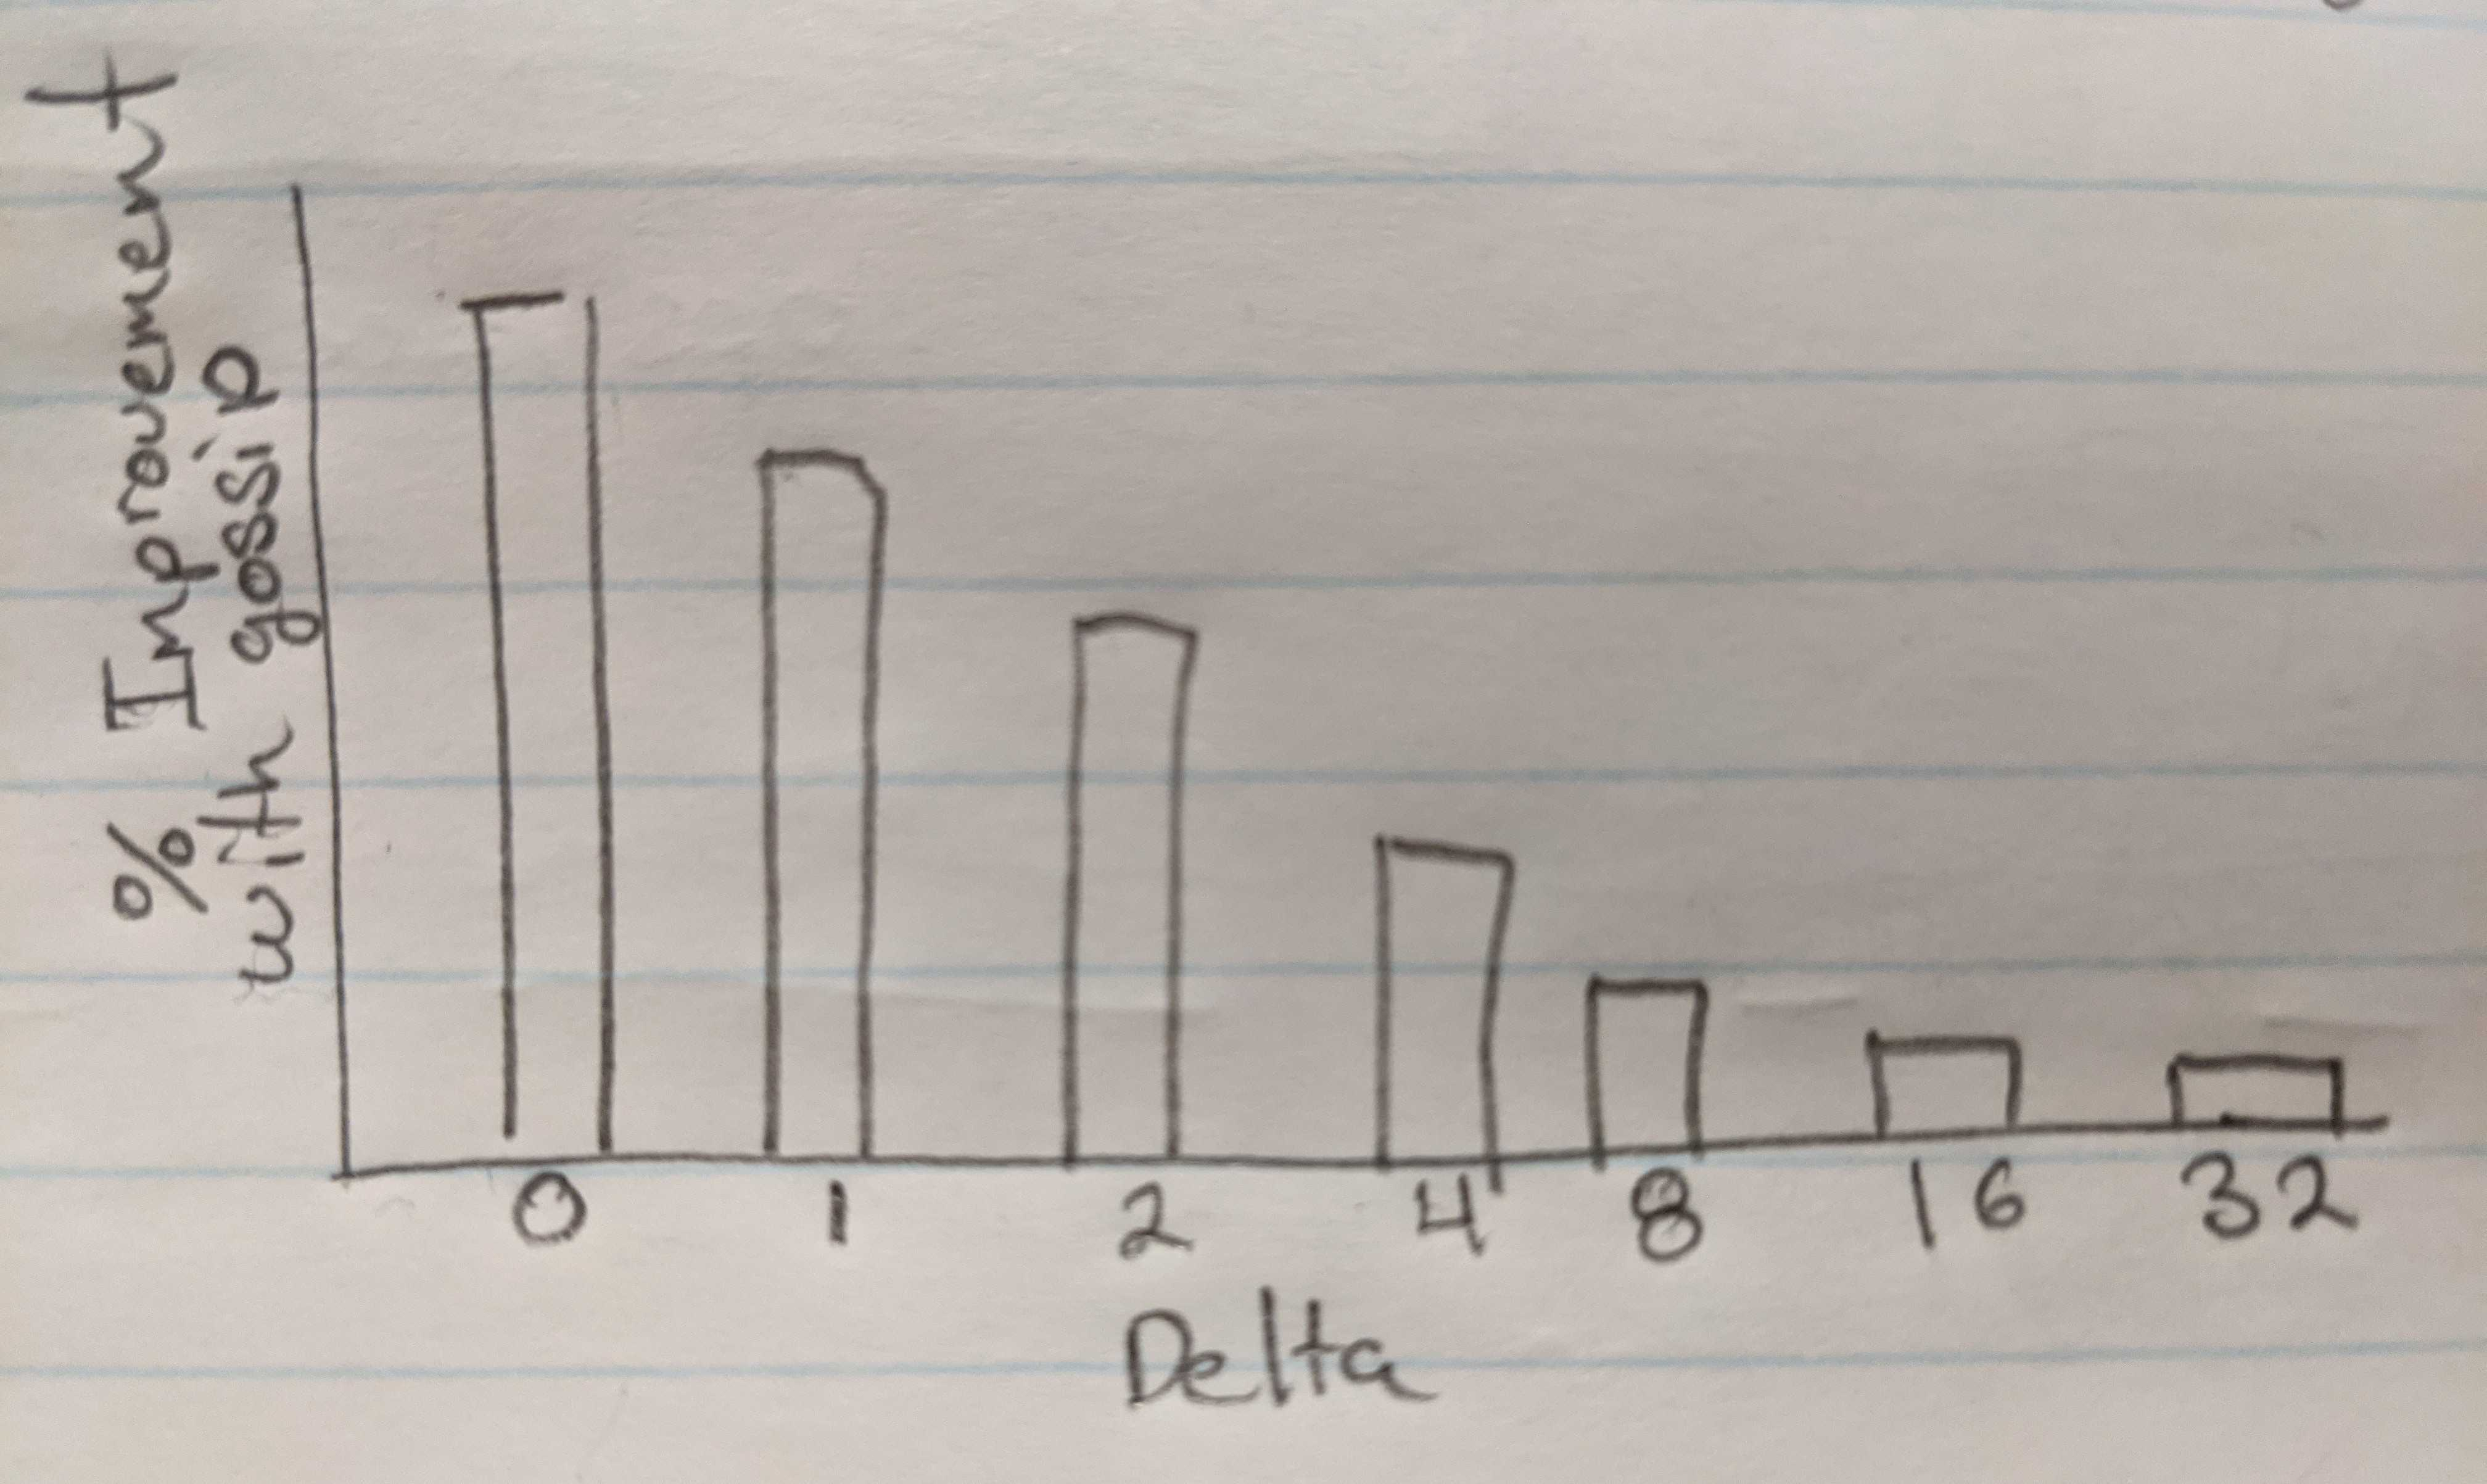
\includegraphics[width=0.45\textwidth]{fig/no_gossip.jpg}
%    \centering
%    \caption{\todo{Percentage improvement in load balancing decisions given
%%    50us load updates}}
%    \label{fig:no_gossip}
%\end{figure}

\subsection{Stale information}

Our experiments show that the frequency at which load is updated has a
significant effect on the quality of the decisions. However, there is a trade
off in terms of traffic overheads to keeping information up to date. As the
number of services increases, so too does the number of messages needed to
keep the information fresh. 

Given imperfect, or stale, information about remote servers, the
question becomes: \textit{when is redirecting requests a good course
  of action}? We submit that given reasonably predictable, but
potentially eccentric, request patterns, the correct course of action
is to act conservatively when conditions are manageable, and to react
quickly and decisively when request loads spike, i.e., in microburst
scenarios.  These constraints dictate a
compromise between inflating traffic and making sub-optimal decisions
with poor information.

\subsection{Information traffic reduction} 

Determining how often and when to send load information requires
careful consideration. If an update were to be propagated for every
request, that would be ideal from a decisions making perspective, but
the overall number of messages sent could inflate by the total
replication factor (2$\times$ or 3$\times$ in many cases).  Such
overheads are unacceptable for systems with requests in the thousands
or millions of requests per second as the cost of the information
quickly surmounts the goodput traffic. A key challenge in designing a
distributed in-network load balancer approach is to identify the most
critical information to send which ideally only produces a small
overhead in terms of state exchange messages.

%\subsection{Predictability}

Network operators generally want predictable behavior within their networks.
Given that distributed load balancing requires information to be spread, it
raises the risk of adding unpredictability to the network, specifically in
terms of overhead. An ideal load-balancing strategy would spread information
efficiently while allowing operators to set an overhead budget in terms of
bandwidth or messages which would correlate to a comparable increase in
performance. Predictability is highly important in heterogeneous systems where
multiple applications require guarantees about their apportioned network share.

\subsection{Heterogeneous rack configurations}

At datacenter scale the configuration for any application may vary wildly.
Individual service replicas may be co-located with resource-hungry applications.
Due to configuration differences applications might have varying processing
powers. Many applications are placed in VMs which execute on differently
powered hardware. Indeed, in the datacenter there is no guarantee that any set
of replicas is equally provisioned. Therefore any load-balancing strategy must
take into account this heterogeneity and apportion requests in response to the
real processing rate.

\section{Daronpon design}

The \systemname\ protocol resides within the ToR at each rack and is designed to
track server load by counting the number of outstanding requests for each
service running on that rack. Figure~\ref{fig:racks} illustrates the role that
ToRs play in our load balancing scheme.  When a request arrives at a ToR it
makes a load balancing decision. It either \textit{Admits} the request, or it
\textit{Redirects} it to another replica. The choice to either admit or
redirect is subject to the local load the service is currently experiencing
under the ToR (as understood by \systemname), and an estimation of the load
each replica has on remote ToRs. 

%If a request is admitted the ToR increments it's
%load counter for that service. Once the server complete the request
%and the response from that service passes back through the ToR the
%load counter is decremented. Each TOR has a perfect count of the
%number of outstanding requests underneath it (assuming reliable RPC)
%which it can use to request count of services running on remote racks
%are sent periodically which give ToRs approximate knowledge of their
%load.  Using this information ToRs make the decision to \textit{Admit}
%or \textit{Redirect} a request when it arrives. 

A ToR can only directly keep an up-to-date counter for the services running in
its rack. To make good load balancing decisions, fresh knowledge, and more
importantly knowledge of bursty behavior, is necessary.  Determining the
mechanisms for disseminating this load information is non-trivial.

We designed and tested a variety of different options for disseminating load
information in simulation and on an Amazon Web Services (AWS) testbed.  One
design gossiped load information periodically based on wall clock time, and
another gossiped on a per-request basis. Our results in simulation and on our
test setup demonstrate that both of these techniques require extremely high
overheads in terms of messages sent.  For example, our best results with
periodic message exchanges required updates polled every 25us. This resulted in
over a 2x overhead in terms of messages. Most of the information spread in this
case was redundant, and does not aid in mitigating bursts.  Further, it adds
congestion to the network, which reduces the maximum throughput, especially
during bursts, which is the opposite of our goal. An ideal load dissemination
protocol would quickly react to bursts while simultaneously generating little
overhead during burst events.

The \systemname\ protocol consists of two distinct but complementary messaging
algorithms.  The first is a logarithmic gossip protocol (described below) which
guarantees the reactive spread of load information when bursts occur, while
generating little overhead otherwise.  The second, an opportunistic
piggybacking protocol, spreads load information between ToRs when requests are
redirected. We find in our evaluation that our log gossip approach prevents
large queue build ups, while our piggyback approach greatly reduces latency in
the common case.  These results are outlined in detail later in this paper.

\begin{figure}[ht]
  \centering
    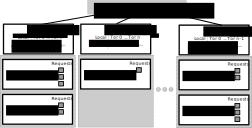
\includegraphics[width=0.8\textwidth]{./figure/daronpon/racks.pdf}
    \caption{High-level overview of \toolname. Each ToR tracks
    outstanding request for services running in its rack, and
    maintains approximate counters for remote ToRs hosting shared
    replicated services.} 

  \label{fig:racks}
\end{figure}

%\subsection{Gossip Periods}
%\begin{figure}[ht]
%  \centering
%    \includegraphics[width=0.45\textwidth]{fig/diffgossip.pdf}
%    \centering
%    \caption{Different gossip periods from 1\/2 RTT to 16 RTTs. Using constant service time 25 us} 
%  \label{fig:diffgossip}
%\end{figure}

%Information about remote load counters is the key factor in making
%redirection decisions. Out-of-date load information is of low utility
%over time as its accuracy decreases. Therefore, the
%load gossip period has a remarkable effect on the overall performance.

%We tested the effect by running different gossip periods.
%After each run the period of gossip messages is doubled, starting at 25 us. 
%Figure~\ref{fig:diffgossip} shows the resulting
%trend when our servers are stressed at 30k request per second. 
%While doubling the gossip period, we can see 
%a linear performance degradation on 95th, 99th, and 99.9th percentiles latency
%starting at 100us, i.e. 1 RTT.
%The 50th, 95th, 99th, and 99.9th percentiles latency increase
%4.4\%, 26.9\%, 42.7\%, 58.3\% with 32x gossip periods. 

%%
%A marginal benefit is found at any gossip periods as a local redirections
%require a queue depths of 1 or greater, and even with poor information
%the probability of a redirected request landing at a less stressed
%server is sufficient enough for a performance benefit. 



% \sg{The aggregate number of gossip messages grows exponentially with the number
% of services running under each TOR. We should consider pointing out
% some mechanisms which might amortize the cost of these messages.}

% \begin{figure}[t]
%   \centering
%     \includegraphics[width=0.45\textwidth]{fig/load_spread.pdf}
%     \centering
%     \caption{ Request latency response to gossip message frequency
%     with servers loaded at 70\%. Exponential increases in frequency
%     lead to linear increase in performance. ~\todo{make off values
%     line up with ~\ref{fig:delta}} ~\todo{average over more runs, this
%     is taken over 10}.
% }
%     \label{fig:load_spread}
% \end{figure}

%\subsection{Load Delta}
%\begin{figure}[ht]
%  \centering
%    \includegraphics[width=0.45\textwidth]{fig/diffdelta.pdf}
%    \centering
%    \caption{Different load delta values to avoid aggressive redirection. Using constant service time 25 us} 
%  \label{fig:diffdelta}
%\end{figure}

%Figure~\ref{fig:diffdelta} shows microbenchmark results 
%of requests latency varies across delta values. 
%Applying ToR redirection with small delta values improves performance. 
%However, larger delta values avoid aggressive redirections but they hurt
%the performance by missing redirection with potential benefits.
%We can see the tail latency substantially increased after delta value of 10 under 
%a 35 KRPS request rate.
%The 50th, 95th, 99th, and 99.9th percentiles latency increase 
%23.0\%, 20.9\%, 13.3\%, and 12.5\% when delta value increase from 10 to 80.

%\begin{figure}[ht]
%  \centering
%    \includegraphics[width=0.45\textwidth]{fig/diffdelta0to10.pdf}
%    \centering
%    \caption{Zoom-in view of delta values from 0 to 10. Using constant service time 25 us} 
%  \label{fig:diffdelta0to10}
%\end{figure}

%As shown in Figure~\ref{fig:diffdelta0to10} increasing delta values
%from 0 to 10, we saw a smaller but observable increase on latency.  We
%observed 22.0\%, 19.9\%, 14.2\% increase on the 50th, 95th, and 99th
%percentiles latency.  The increase on 95th, and 99th percentiles
%latency starts at delta value = 5.

%We saw a local minimum of request latency at delta value 2 and 3 at medium request rate 30kRPS.
%Using delta=2 gives us 7.1\%, 8.2\%, 7.8\%, and 7.1\% improvements on
%on 50th, 95th, 99th percentiles, and 99.9th percentiles. Throughout
%our experiments we use a delta value of two as our local optimum.


%\todo{Load delta can be used as a way to reduce the total number of
%packet redirections. Should we choose to add redirections to the cost
%of our algorithm we want to show how using a load delta can decrease
%that}

\subsection{Microbursts}

Figure~\ref{fig:microburst} (top) shows an example of a microburst. In this
case, requests are issued at a Poisson arrival rate by multiple clients.  The
peaks show outstanding requests from the perspective of a ToR instrumented to
track request counts. In this case, when requests queue, that queue grows
without bound, even though other replicated services are available to process
this influx of requests. This has a dramatic impact on the tail latency of the
requests in the burst, and also the overall mean request time. A typical
request incurs longer wait times due to decreased overall system throughput.

In Figure~\ref{fig:microburst} (bottom) the queue builds up with our
logarithmic gossip mechanism enabled. Each \textit{red X's} on the chart
represents a point at which the load on the server is gossiped.  Note that when
peaks occur, and a gossip is sent, the load is quickly spread to other servers.
This increases overall system throughput and decreases tail latency. This
strategy, however, is not perfect. At low load the benefit of redirecting
requests is minimal. For example, when the number of outstanding requests is
just one or two above a remote service, and so redirection reduces overall
performance.

The age of the gossiped information complicates the act of redirecting. The
remote information on remote hosts is at least a few microseconds out of date.
Given the few microsecond budget our requests have to begin with, the benefit
of redirection quickly evaporates if even a few request arrive from the point
in time at which the load information is sent.  This leads to unnecessary
redirections and high overheads in terms of gossip messages which do not
ultimately deliver useful information. This overhead can be mitigated by adding
a threshold which prevents gossip messages from being sent until the number of
outstanding requests has exceeded a given threshold.  Our proposed log gossip
technique for curtailing this overhead is described in the following section.

%Gossip messages consume and packet processing time.  Therefore their
%frequency must be chosen with care as to not introduce significant
%variance into the system. The majority of data center packet drops
%occur on south facing ToR egress to the host.~\cite{jupiter-rising},
%our approach only increases bandwidth above the ToRs which allows for
%a higher gossip bandwidth budget prior to it causing significant
%interference. Gossip messages are small, (approximately
%64 bytes depending on the number of services), which reduces aggregate
%bandwidth consumption.

%Our testbed results use gossip messages as
%frequently as 10us without any noticeable interference on 40Gbps
%networks. As network speeds increase we anticipate that the available
%bandwidth for background traffic which improves the performance of
%running services will increase.


\begin{figure}[t]
  \centering
    \includegraphics[width=0.80\textwidth]{./figure/daronpon/burst.pdf}
    \centering

    \caption{Microburst with no mitigation (top) vs. with
    logarithmic gossip load balancing enabled (bottom)}

  \label{fig:microburst}
\end{figure}

\subsection{Packet flow}

The \systemname\ load balancers are stateful and act per request.
Figure~\ref{fig:load_balancer} provides a high level message flow diagram of
this system.  When requests arrive, \systemname\ executes the admission
protocol. Requests are admitted only if the local service has the minimum
observable global load. A load tracker keeps counters for each global service.
Local counters are up-to-date, while remote counters are learned via gossip and
piggyback messages.  When a request is admitted, the ToR increments its load
counter corresponding to that service.  When a response passes back through the
ToR, that service has its local counter decremented.  If, when a request
arrives, the local load of a service is not the global minimum, the request is
redirected. The redirected request is then sent to the service with the lowest
load, based on the ToRs' local load tracker (see
Section~\ref{subsec:piggyback}).  Redirected requests have load information
attached to them. The attached load consists of request counters for the
intersection of services the ToRs share.  Therefore, the overhead per
redirected request is variable as per the systems' configuration.

Increments and decrements in local load are tracked by a gossip monitor (see
Section~\ref{subsec:gossip}). The job of the gossip monitor is two-fold. First,
it identifies bursts. When load spikes the monitor broadcasts gossip messages
to let other ToRs know it is experiencing high load. Second, it identifies
valleys. Load balancing schemes which use potentially stale information are
known to exhibit herding behavior, a condition which leads to sub-optimal
queuing behavior~\cite{dahlin_stale_info,mitzenmacher_old_info}. When load
drops sharply, gossip messages are also generated to announce that a service
has spare processing capacity.

\begin{figure}[t]
  \centering
    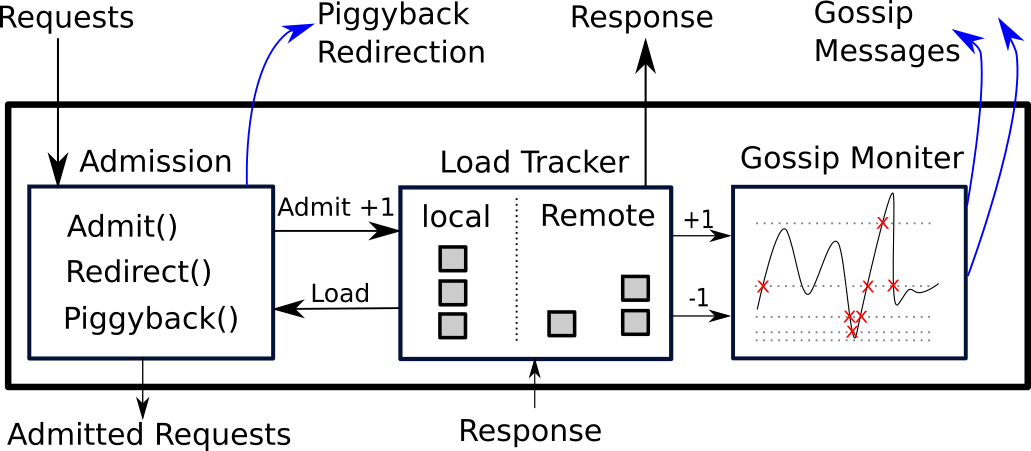
\includegraphics[width=0.80\textwidth]{./figure/daronpon/load_balancer.pdf}
    \centering

    \caption{ %% 
        %%
        Key functionality and message flow of \toolname.
        Incoming requests are either admitted or redirected.
        Redirected requests spread load information via piggyback.
        Load is updated upon admission, and response.  Gossip messages
        are issues when load breaks a logarithmic threshold.}

  \label{fig:load_balancer}
\end{figure}

\subsection{Logarithmic Gossip}
\label{subsec:gossip}

\begin{figure}[t]
  \centering
    \includegraphics[width=0.90\textwidth]{./figure/daronpon/log_thresh.pdf}
    \centering
    \caption{The percentage of gossip messages generated by a
    logarithmic gossip mechanism as a percentage of overall traffic.
    Collected from runs of 96 KRPS.} 
  \label{fig:log_thresh}
\end{figure}

The \systemname\ algorithm for generating gossip messages has the primary goals
of reacting quickly to bursts while consuming little overhead in terms of
additional messages.  In an earlier design, ToRs gossiped load information every
25 $\mu$s. This approach has the advantage of providing highly updated load
information, but it incurred scalability bottlenecks as the number of ToR
increased, since the 25 $\mu$s gossip contends with request goodput for link
bandwidth.

To compress the number of messages, we adjusted the gossip protocol to only
send messages on exponential changes in load. We use powers of two as our
exponential interval, and we choose two both for its effectiveness in practice
and for its ease of computation, only requiring bit shift operations. To our
knowledge, no commodity programmable switch can compute floating point
arithmetic in the data path~\cite{challenging_programable}.

Each exponential step increases the bounds in which server load can fluctuate
prior to a gossip message being issued. For instance, if the load were to
increase from 1 to 2, a gossip message would be broadcast to all other servers
with the replicated service that crossed this threshold. In this message, load
information for all other shared services is added. When the boundary of two is
crossed, and the value of two is sent, this ToR will not issue another gossip
message until the load on the service rises by a power of two to four, or falls
back down by a power of two to one.

%%
%% Sorting microbursts by size
%%
The above described protocol has several benefits. First, it sorts microbursts
by magnitude without adding significant packet overhead. Given that small
fluctuations may occur at rapid pace, it is important to give priority to
bursts with larger magnitudes. Other methods of achieving this goal such as
piggybacking can lead to stale information, which has significant differences
to ground-truth values, even when a server is experiencing very
high load.


%%
%% Reduces congestion when bandwidth is needed
%%
The protocol also decreases the number of gossip messages sent during 
bursts, which reduces the overall strain on the system when resources
are at their tightest. This is an issue with gossip strategies that
operate periodically (e.g. at preordained wall clock times)
or are issued at some constant ratio
to requests (e.g gossip every 5 requests).  When request rates
are low, gossip messages are automatically sent with a higher frequency
per number of requests which allows for better decision-making at lower
request rates.
%%
%%Aggregation of requets
%%
ToRs have the advantage of being an aggregator for the load of an
entire rack. Were we to implement our solution on end hosts, each host
would need to gossip its load to every other host. Using ToRs, the load of
each server in a rack is known explicitly and is gossiped in its
entirety, assuming the rack sees both requests and the associated
responses.

%%
%% Fast reaction
%%
Other approaches which use load information collected from end hosts
themselves suffer from additional delays in responding to load spikes,
as the knowledge of load must be transmitted to the balancer before it
can react. Our approach reacts to load as soon as a request is
admitted. This allows for precise load balancing decisions to be made
at sub-RTT time scales. 
%%
For instance, in a Fat-Tree with two ToRs connected by a single
aggregate switch, the distance traveled by load updates is halved in
comparisons to a host based solutions (e.g. Tor-Agg-Tor vs
Host-Tor-Agg-Tor-Host). This approach is not limited to Fat-trees,
as
many networks use ToRs, however our ToR-based approach always results
in two hops less than an host based approach.

%% %Approximate measure of load, but fast react %
We give up precise, up-to-date measures of load on the host, something we can
only get with precise application level knowledge and host control, and instead
use counters to estimate server load in the ToR. This imposes lower tracking
overhead, and performs nearly as well as highly tuned approaches which report
server load directly~\cite[Figure. 15 (proactive)]{racksched}.

%%
%% Threshold
%%
This algorithm decreases the number of gossip messages
significantly, and can be greatly improved by carefully considering a
lower bound at which to disable the mechanism entirely.
For example, setting a lower
threshold such as $t$ implies that below an outstanding request count of
$t$ a ToR will not gossip information.


Figure~\ref{fig:log_thresh} shows the percentage of messages gossiped relative
to the requests processed for different threshold values.  Note that the
default values of 0 and 1 have an overhead of around 30\% of the request rate.
Redirections of requests at these levels of outstanding request sees little
benefit in terms of performance as at any reasonably high request rate, the
depth of remote queues have changed since the remote data was received making
the choice stale. By increasing the threshold to four, the overhead in gossip
messages is reduced by a factor of ten down to around 2\% when our system is
around 70\% saturation. See Section~\ref{sec:service_time} for a comprehensive
evaluation of gossip overhead. Increasing the gossip threshold beyond four
significantly reduces overhead down to around 0.02\%, however this comes at the
cost of only identifying bursts of size eight and greater which significantly
effects our reductions in 99th percentile tail latencies.

%%
%% Staleness
%%
One limitation of our algorithm is that it provides no liveness
guarantees with regard to the freshness of the load information
announced. For instance, a server which maintains an outstanding number
of requests between 4 and 16 for $n$ requests will not issue a gossip
until either threshold is crossed. While this is unlikely in practice
due to the small range and short duration of requests, there is no
guarantee. This can become an issue for extended periods of load when
the number of outstanding requests is deep (e.g. 128 to 512).

\subsection{Piggyback}

\label{subsec:piggyback}
\begin{figure}[t]
  \centering
    \includegraphics[width=0.90\textwidth]{./figure/daronpon/breakdown.pdf}
    \centering
    \caption{Performance breakdown of gossip and piggyback mechanisms.
    Lower values are better.} 
  \label{fig:breakdown}
\end{figure}

Using logarithmic intervals for gossip messages, we can clearly identify and
mitigate bursts.  While this is advantageous in general, there is still
additional performance to be gained.  With gossip enabled, the percentage of
redirected requests is around 22\%. Each one of these redirected requests is
sent from the redirecting ToR to the receiving one, and therefore has the
ability to report the load information on the ToR that performed the
redirection.  We refer to this method of attaching load information to
redirected requests as piggyback, and using redirection to spread information
provides significant advantages in the common case.

In contrast to the centralized approaches in both Racksched and
R2P2~\cite{racksched, r2p2} piggybacking information load on requests
is not a sufficient mechanisms for learning about remote load. This is
because our load balancer is decentralized, which means that our load
balancers do not see load information updates from every request.
Unlike our logarithmic gossip mechanisms, it provides no guarantees
about its operational bounds. Using gossip messages exclusively
provides no guarantees that any specific server will have information
propagated to it as only the server which is redirected to receive
fresh information.

In the case of these centralized solutions, each request returns some
information to the scheduler. In the distributed case, there is no liveness
guarantee with regard to redirections, and indeed, information can become
arbitrarily stale. We therefore consider our piggyback algorithm to
opportunistic, only aiding in the common case when load is low, but when making
precise redirections will still improve throughput and provide
lower latency.

Piggybacking load has the advantage that it is responsive proportional to the
request rate of the system. As the number of requests per second increases so
to does the rate at which information is spread between ToRs. Further, it has
the advantage of introducing a small amount of overhead. Rather than incurring
the cost of an entire load information update, this only adds a few bytes to a
custom header injected at the ToR.

Figure~\ref{fig:breakdown} shows a performance breakdown of the two parts of
our protocol. At low request rates the gossip protocol does not provide much of
a performance benefit in relation to the piggyback method. However as the
request rate, and variability, of the system rises (e.g. to 102 and 105
thousand requests per second), the gossip mechanism provides the majority of
the gains as it detects the peaks which increase tail latencies the most.

\section{Implementation}

We have deployed \systemname\ in the AWS cloud environment, with service
instances hosted in VMs connected via Elastic Network Adapter (ENA) virtual
NICs. These instances use the Data Plane Development Kit (DPDK).

\paragraph{Components:} Our deployment consists of three components: DPDK ToRs,
DPDK clients, and servers with default Linux networking stacks relying on UDP
for application messaging. DPDK is a kernel bypass networking library which
allows for high throughput and low latency packet processing in user
space~\cite{dpdk}. DPDK ToRs emulate ToR switches with limited latency overhead
($<$ 1 microsecond).  Ideally, we would implement our algorithm on P4 switches,
however to our knowledge no cloud providers allow for customers to offload
custom programs to programmable switches at this time.  We implement our
clients using DPDK for lower latency and precisely controllable request rates.
These traits are important as AWS's ENA NICs do not have hardware timestamping
available to users.  Our DPDK clients can generate hundreds of thousands of
requests per second with a single virtual core. These UDP-based servers
represent services relying on the standard Linux networking stack. We choose to
use UDP as the transport because it allows us to redirect request atomically
without connecting multiple packets together and redirecting as a group, though
this could be supported as future work.

\paragraph{\toolname\ DPDK ToRs:} Our DPDK ToRs use an arbetry number
of cores to forward requests/responses and a single core to gossip
load information. Redirecting involves header manipulation, tracking
load information using hashtable table lookups, and counter
increment/decrement operations. The operations we used in these DPDK
ToRs are carefully chosen to be simple, and within the capabilities of
programable switches to compute.

\paragraph{Custom packet headers:} We our inject custom header after
the IPv4 UDP header. It consists of a unique request ID for each
request, which is used to track lost packets and measure end-to-end
latency. A service type field differentiates services, e.g Memcached
and RocksDB.  Additionally, the IP and ports describe addresses of
replicas which implement other copies of the service.  We assume that
clients know the server replica addresses by asking the cluster-level
replication manager, e.g., Google's Slicer or Facebook's Shard
manager~\cite{facebook_shard,google_slicer,microsoft_service_fabric}.
Gossip messages are also based on UDP, and load information is
appended after the UDP header.  The header contains a list of server
addresses, load counters, and its corresponding service types for all
servers under a ToR switch. 

\section{Evaluation}
\label{sec:eval}

%define setup variables here
\newcommand{\instances}{9 }
\newcommand{\racks}{3 }
\newcommand{\servers}{3 }
\newcommand{\servercores}{1 }
\newcommand{\tors}{3 }
\newcommand{\torscores}{8 }
\newcommand{\clients}{3 }
\newcommand{\clientcores}{1 }

We evaluate \systemname in on the Amazon Web Services cloud (AWS
\texttt{us-west-2} region). In this section, we describe these experiments and
the resulting conclusions.

\subsection{Experimental setup}

%\textbf{Testbed:} %
We use \servers \texttt{c5n} instances as servers, \clients as clients, and
\tors as software ToRs. All instances are placed in a single cluster placement
group for predictable low latency. The mean RTT latency between every instance
is about 50 microseconds.  In this setup, we configure three server machines,
three clients, and three DPDK software ToRs. This simple configuration emulates
a datacenter network in which each ToR has exactly one service running
underneath it.  Services are deployed to servers using the stock Linux
networking stack.  While this does incur higher latencies as compared to
DPDK-based kernel bypass stack, we note that it is representative of many
datacenter applications.

%why did we chose to do it on AWS?-> it's a real cloud  why did we
%chose to use DPDK software ToRs-> because we don't have access to the
%ToR to make latency more tractable we use cluster placement group

We implement the \textit{random} service selection as a simple and standard
baseline. Client-based ``power of two'' approaches are not comparable because
they require excessive probing of server load, incurring at least one RTT per
probe. This load creates unnecessary congestion on the DPDK ToR instances and
ENA virtual NICs.  \toolname\ can be easily extended to implement the ``power
of two'' approaches on ToRs and the performance should be similar, based on
simulation results reported in LSQ~\cite{lsq}.  Each client randomly selects a
service designation. In the random configuration, requests traverse our DPDK
software ToRs with our load balancing mechanism off, and they flow through to
their selected destinations. We compare \toolname\ random in
the following experiments.

\subsection{Workloads}

We evaluate our load balancing approach with a simple request-response
application, in which the time spent on the server is computed based on a
statistical process.  In our evaluation, we generate requests according to two
statistical distributions, one of which generates application-level requests
and is run on DPDK-based clients, and another which generates emulated service
times. Clients generate requests based on open-loop Poisson arrival using the
standard random library.  Servers distributions are split into different
distribution categories, each of which has its own separate parameters. These
include constant time, bimodal, and exponential distributions. 

Each server is loaded with an equal number of requests (in expectation)
drawn from common request rate distributions, as described next.
Our goal in using these distributions is to demonstrate that
our technique of using outstanding requests (blind to the underlying
service distribution) works in general, without the need to tune
our load balancer for each application.  Both our gossip protocol and
piggyback protocol are enabled in each experiment. The lower threshold
on our gossip protocol is 4.

\noindent\textbf{Constant:} In this distribution, all requests take 25 $\mu$s to
complete on the server.  In the server, a work thread busy-polls the time until
the 25 $\mu$s deadline has passed to emulate application-level service times.
This workload is indicative of many highly tuned key-value stores with strict
SLOs~\cite{memcached,rocksdb}.  Our servers experience additional latency
overheads from the Linux networking stack.  Our choice of this constant latency
is intended to be representative of a performance-tuned microservice which
performs a fixed amount of work per request.  To provide a sensitivity analysis
to this choice of constant, Section~\ref{sec:service} provides an overview of
our system performance across constant service times separated by an order of
magnitude above and below 25us.

\noindent\textbf{Exponential:} To generate an exponential distribution we use the
standard C++ random library. We set the mean to 25 $\mu$s with a standard
distribution of 40,000. These parameters generate tails of up to 400 $\mu$s
which is indicative of many applications that may be subject to blocking, such
as occasional writes to disk or the invocation of a blocking RPC to another
machine.

\noindent\textbf{Bimodal:} Our bimodal service times are distributed into two
categories. 90\% of the requests take 13 $\mu$s and 10\% are 130 $\mu$s.  We
choose this distribution as the mean value is close to 25 $\mu$s. This
distribution is aimed at emulating longer and less frequent tasks such as
writes and scans in certain key-value store workloads or even garbage
collection events in the runtime.

\subsection{End-to-end experiments}

\begin{figure*}
  \includegraphics[width=\textwidth,height=4cm]{./figure/daronpon/homo.pdf}
  \caption{99th percentile latency improvements on three common
    service distributions (Constant, Bimodal, Exponential). Each
    server is provisioned with homogeneous processing power.}
  \label{fig:homo}
\end{figure*}

We test the effectiveness of our load balancing technique by running it against
random replica selection alternatives on the aforementioned workloads.
Figure~\ref{fig:homo} shows the relative performance gains across these
workloads at the 99th percentile latency. In this configuration, each of the
servers has identical processing capacity for each service.  We consider this
idealized and homogeneous configuration because of its simplicity.

\systemname sees the most relative gain over random when skew in the workloads
is common. At high loads, request variation occurs at higher degrees for
multiple reasons. First, the Poisson arrival process on our clients has a
higher probability of generating bursty sequences of events at higher load.
Second, hypervisor and NIC hardware on AWS contributes to the bursty arrival of
requests because of the underlying batching behavior.  These forms of
burstiness is largely out of our control as we do not have direct access to
AWS's hardware configuration.  Finally, as rates increase, more batching
happens in the Linux kernel networking stack. This leads to sharp decreases in
the number of outstanding requests. 

\toolname\ sees the largest benefits in the bimodal and exponential
distributions and the long service times cause significant and frequent queuing
on the end hosts. The logarithmic gossip protocol reacts quickly to these
changes under load and steers requests away from the servers which are running
long average request times.  In our homogeneous experiments, the average value
for number of outstanding requests is four in our constant distribution, with
frequent peaks of up to 80 outstanding requests when \toolname\ is disabled.

\noindent\textbf{Constant:} Figure~\ref{fig:homo}A shows our approach provide benefit
on tail latency starting at 78 Krps (kilo-requests per second).  This constant
workload gives \toolname\ the fewest opportunities to load balance effectively
as the random distribution of requests, each with a static service time, should
be approximately even. In this distribution, the benefit is found in the load
fluctuations. At high request rates, other mechanisms such as Linux's request
batching, have more of an effect on queuing.

At the highest request rate that a single vCPU core can handle, the latency
improvement of \systemname at the mean is 1.32x and on 99.9th percentile is
1.62x.

\noindent\textbf{Bimodal:} In Figure~\ref{fig:homo}B, we see the disparity between
random service selection and \toolname. The service time dispersion provided by
bimodal distribution causes noticeable request queuing when a long service time
request occupying a service.  Logarithmic gossip messages are ideal in this
case as they quickly react to the skew in load.  Further, in this distribution
the probability of finding an under-utilized replica is relativity high.  

\noindent\textbf{Exponential:} Figure~\ref{fig:homo}C shows the throughput and
latency gains on an exponential server distribution. Our benefits are most
noticeable here as the exponential distribution leads to the fastest disparity
in load. In this case, a single request on the exponential distribution can
lead to significant queuing on a given server. Our latency improvements at 102
Krps is 1.61x in the mean and 1.54x at 99th percentile.

\subsection{Heterogeneous server configurations}

\begin{figure*}
  \includegraphics[width=0.9\textwidth,height=4cm]{./figure/daronpon/hetero.pdf}

  \caption{Throughput and latency improvements with skewed processing
    capacity in a heterogeneous server configuration. \toolname\
    scales linearly with with the aggregate processing capacity
    available.}

  \label{fig:hetero}
\end{figure*}

The placement of replicated services is subject to the cluster
scheduler~\cite{facebook_shard,google_slicer,microsoft_service_fabric}.  The
placement of individual services may be tightly coupled to a single rack, or
distributed to multiple racks.  Additionally not all replicated services may be
configured using identically powered instances. Some may be provisioned with
different core counts, memory, and potentially different OS versions.  Finally,
should rack-level scheduling be utilized such as Racksched or R2P2, the
individual rack level throughput may differ below the operating domain of
\toolname.

To show the generality of our approach in situations where replicated
applications differ in their throughput capabilities, we configure one out of
our three servers to run using twice the processing capacity (i.e., two CPU
cores rather than one). In this setup, clients otherwise operate identically to
the homogeneous configuration.

Figure~\ref{fig:hetero} shows the performance gains from enabling \toolname\ on
our heterogeneous testbed. In this test, the server with twice the processing
power of the other processes requests twice as quickly.  Our random client
takes no measure of queue depth, and therefore does not adjust to this excess
compute power. Its performance is only marginally better in this case, as the
request which its probabilistically sends to the doubly provisioned server are
processed more quickly. 

\toolname\ apportions load to servers in precise relation to their processing
power. Our results from this test show that \toolname\ exhibits ideal scaling
in this small test. Where three vCPUs can process about 100Krps, four can
process about 133 Krps with the same 99th percentile tail latency. When running
in a heterogeneous configuration, the proportion of gossip and piggyback
request remains approximately the same as in the homogeneous case. The gossip
mechanism is triggered periodically as the request on the faster servers drains
below its current threshold, however this periodic variance occurs on the same
order as the natural fluctuations in load. Redirections also occur at
approximately the same rate, however they are almost entirely directed at the
over provisioned server.

Ideally, we would demonstrate the scalability of \toolname\ across many racks
with more services. We see this heterogeneous result as a proof of concept that
our approach can scale approximately linearly with available processing power.
We expect this result to hold as our approach is similar in style to
theoretical approaches for distributed load balancing which are proven to
provide linear scaling while using incomplete local information to balance
load~\cite{lsq}.

\subsection{Service time sensitivity analysis}
\label{sec:service_time}

\label{sec:service}
\begin{figure*}
  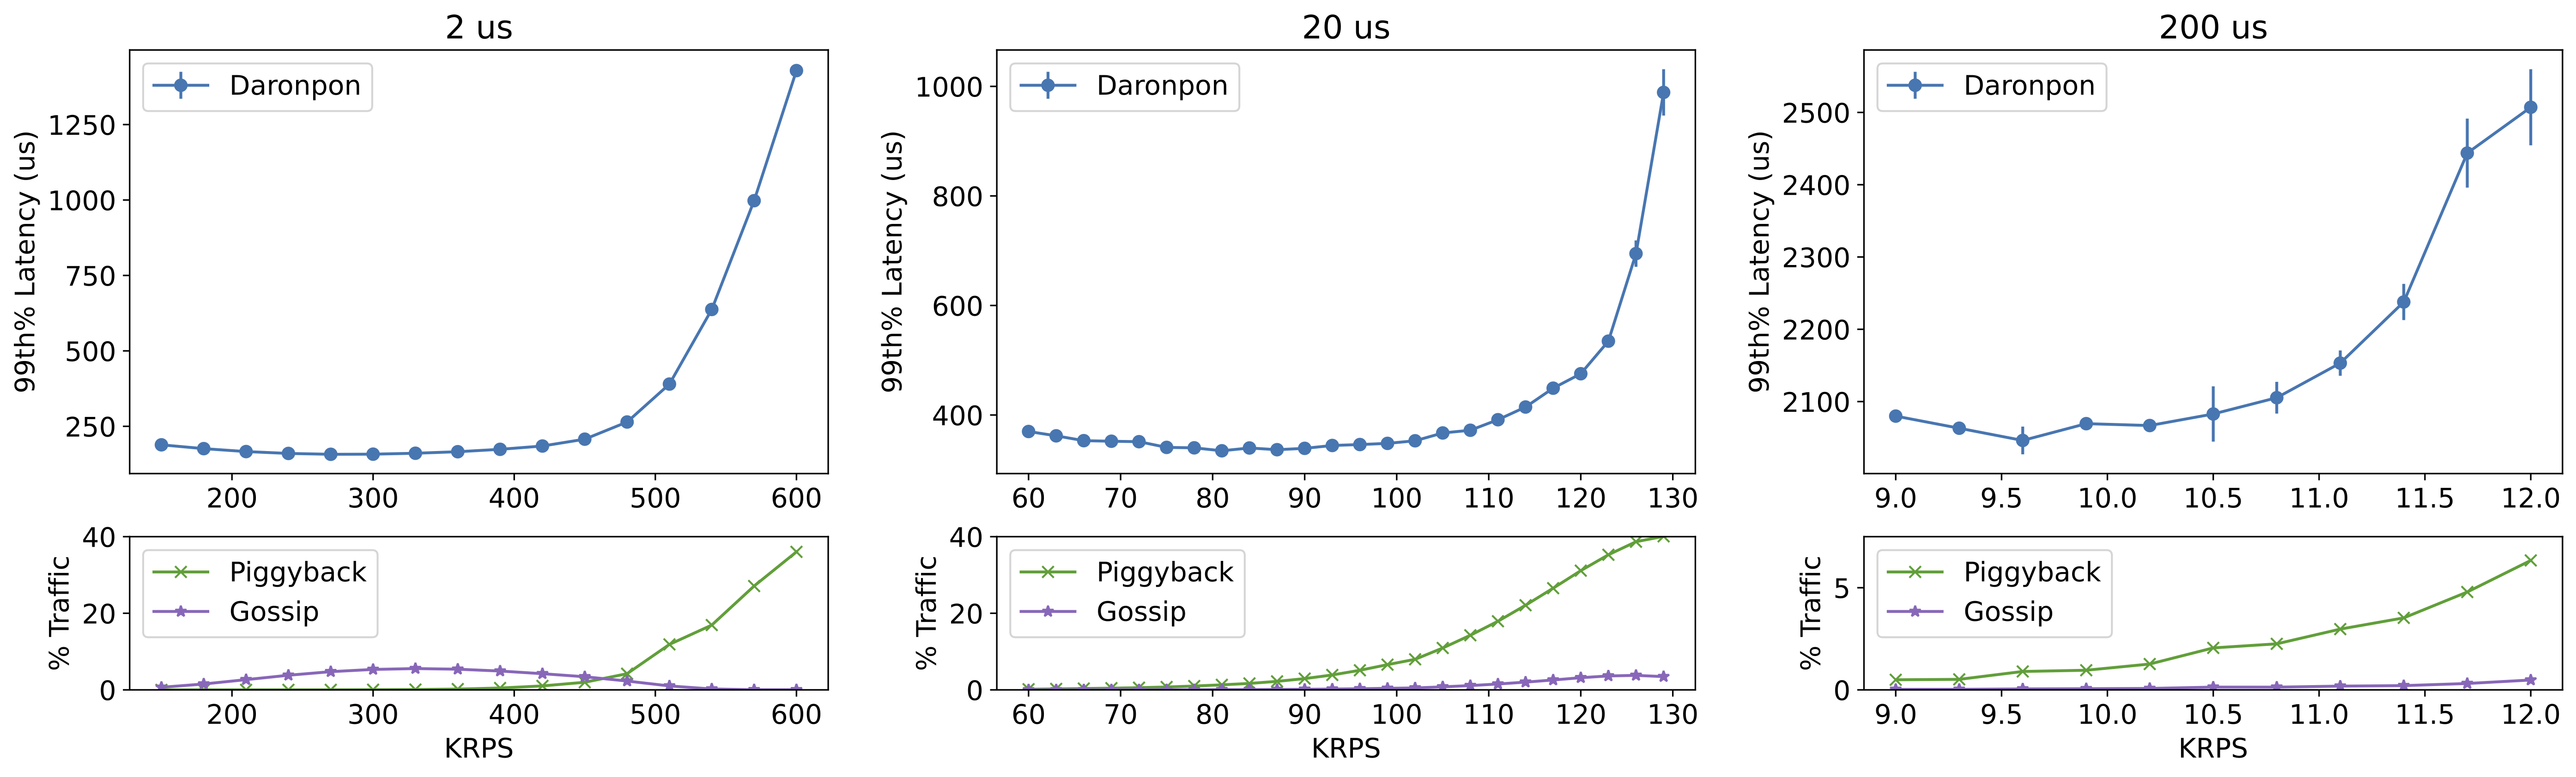
\includegraphics[width=\textwidth,height=4cm]{./figure/daronpon/service.pdf}

    \caption{Service times across three orders of magnitude (2us, 20us,
    200us). \toolname\ provides relative improvements with similar
    overheads in terms of piggyback and gossip messages at each
    service time. 
    \TODO{This needs to be changed to EWMA results along with the text.}
    }

  \label{fig:service}
\end{figure*}

We choose 25 $\mu$s as a baseline service time for an example microservice,
however our load balancing techniques are not limited to timescales centered
around this constant. To demonstrate that \toolname\ can provide throughput and
latency improvements across differing service times, we vary a constant service
time by three orders of magnitude across three experiments: 2 $\mu$s, 20
$\mu$s, and 200 $\mu$s.  Lower mean service times mean that our Linux servers
are able to process more requests per second, and vice versa.  It also means
that the number of outstanding requests from the view of our software switches
is higher on average.  We show the effect this has on the logarithmic gossip
mechanism, and the proportion of messages which are redirected at each request
rate.

Figure~\ref{fig:service} shows the performance gains \toolname\ achieves in
each case. At 25 $\mu$s (see Figure~\ref{fig:service}, middle), our mechanisms
operate as shown in prior experiments with the maximum gossip overhead reaching
no more than 3\% at peak system load. The number of piggyback messages grows
with the request rate. This is because at higher rates more bursts occur, and
thus the opportunities to load balance increase.

Near peak load, the number of redirections reaches approximately 40\%, and
while this results in the highest performance, it does incur an additional tax
on link bandwidth. We devised a threshold similar to the baseline used in our
log gossip mechanism which required the value of a remote queue to be lower
than that of the local queue by a specified delta before a redirection occurs.
In each of our experiments, this delta value is set to 0, which means that the
minimum replica is always selected. Choosing delta values above 0 resulted in
significantly lower numbers of redirections, with a value of 8 resulting in
piggyback messages being generated around 6\% of the requests, but also
resulting in only a 4\% performance gain over the random policy. In this way,
redirection mitigation is a strict trade-off of performance, resulting in lower
tail latencies at the cost of additional bandwidth.

At 2 $\mu$s, \toolname\ provides less relative improvements than at 25 $\mu$s.
This is due to the increased average queue depth, and the effect it has on our
log gossip mechanism.  Statically, using powers of two as a means to compress
the number of messages is worse in this case than when the outstanding requests
are lower. This is because at lower thresholds powers of two are exceeded more
frequently. At ranges of 64 and above, bursts need to be quite significant
before they result in a gossip exchange.  As seen in the lower part of
Figure~\ref{fig:service}, 2 $\mu$s gossips as a percentage of the overall
traffic starts to fall around 300 Krps.

Here we consider that an additional mechanism such as adjusting our baseline
for gossiping based on an exponentially weighted moving average rather than a
constant could produce higher performance gains and better burst resilience at
high rates. EWMA have been used on programmable data planes in the
past~\cite{adaptive_planes}. We do not explore this mechanism in depth for the
sake of simplicity, and because our power of 2 log approach continues to
operate with benefits at these rates.

At 200 $\mu$s service times, \toolname\ provides slightly better performance
relative to the 25 $\mu$s as information on the servers is likely to stay fresh
for longer due to the decreased request rate.  The latencies at request rates
lower than 9 Krps are higher because interference from the Linux kernel which
starts to reschedule cores below that threshold~\cite{mutilate}.

In all cases the overhead from logarithmic gossip remains low, and is able to
quickly detect bursts. When request rates are high, average request
latency is largely improved from the increase in redirected messages
which provide ample fresh load information which allows for more
accurate predictions of the globally shortest service queue.

\section{Discussion}
\label{sec:discuss}

\paragraph{Scaling:} In production cluster, managers determine the application
service replication factor. This factor is determined dynamically by monitoring
system load, which can cause applications to scale up and down significantly on
the order of hours.  \toolname{}'s gossip broadcast is inflated by this
replication factor, and therefore very large replication counts (e.g. in the
100s) present a potential bottleneck.  We believe that overhead can be
constrained with proper placement of services to maximize the intersection of
services across a same set of racks.  Additionally, careful placement enables
piggybacking to carry more load information per redirected request.

\paragraph{Emerging Topologies:} \toolname\ works on any datacenter topology
which uses ToRs, or virtual ToR-like abstractions (such as our DPDK software
middlebox switches). Emerging network designs, e.g. Jellyfish~\cite{jellyfish}
and Xpander~\cite{xpander}, are supported under our architectural assumptions.
Some network designs have asymmetric latencies between servers.  While this may
cause some racks to propagate information which is more stale, we do not see
this as a limitation of our techniques as our AWS testbed has latency variations
on the order of a few microseconds.  \toolname's redirection piggyback and load
gossip can take a variable amount of time to propagate load information to
other ToRs, but our load balancing design is similar to theoretical techniques
prevent to be effective even with stale information~\cite{lsq}. 

\paragraph{Budget:} We set gossip thresholds statically, which makes
them vulnerable to antagonistic request patterns. With a threshold of
four, gossip can be constantly triggered by a client issuing 4-packet
bursts, leading to an overhead of 25\% rather than 2\%. We consider
two strategies for adjusting our use of gossip. One is maintain an
exponentially weighted moving average of the request rate, and
configure gossip to trigger at a logarithmic deviation from the mean;
allowing gossip to adjust proportionally to average request rate. An
alternative would be to allow operators to set a budget for the
percentage of gossip traffic.  Gossips could be
weighted by priority: a gossip of load 16 is higher than 4,
and the probability of issuing it would be hinged on the number of
messages sent in recent history. Such configurations are not free,
and would be configurable at the cost of performance.

\section{Limitations}

\paragraph{Multi-packet requests:} \toolname\ operates on IPv4 UDP packets. We
do not build reliable transport into our protocol and assume that
retransmissions of lost requests are handled by the application. To support
reliable transmission such as TCP \toolname\, we would need to track
flow-specific state in the network and ensure that once a replica is selected
for a request, no further selections occur on that flow.

\paragraph{Failures:} Our approach does not explicit handle failures. If a
server fails, \toolname\ will automatically load balance around it, as requests
issued to the failed server will not respond, and thus the queue will grow
indefinitely. If a \toolname\ ToR were to fail, that rack becomes partitioned.
We leave the detection of ToR failure in this case to future work.

\paragraph{Application Heterogeneity:} \toolname assume that all replicas are
created equal, in that any request can be sent to any replica. In the case of
replication systems with various roles, such as leaders and
followers~\cite{raft}, additional application-level information would be
required to only perform replica selection on requests which do not have a
specially configured destination.

\section{Future Work}
\label{sec:future}

We've used DPDK as a software ToR for simplicity. The latency between our
software switches is approximately 25 $\mu$s on AWS.  This overhead is caused
by the underlying network at AWS. Due to our gossip-based protocol, every
microsecond matters when making load balancing decisions, with lower latency
improving our results. In the future, we would like to implement \toolname\ on
a P4 switch such as the Barefoot Tofino 2~\cite{tofino2}. We predict that with
inter-ToR one-way latencies between 1 and 3 $\mu$s, our load balancing
decisions will greatly improve.  Also, thus far we've explored microservices
which we expect to have service times on the order of tens of microseconds.
Recent work in persistent memory has demonstrated that remote storage is now
accessible on these same time scales, and so we believe that replicated storage
might benefit from our approach to load-balancing.

\section{Conclusion}
\label{sec:conclusion}

In this work we present \toolname, a microsecond time-scale load balancer for
replicated data center-wide applications.  We have developed a novel hybrid
gossip and piggyback synchronization protocol to keep ToR switches synchronized
with application load with low overhead, and have demonstrated the
effectiveness of this technique by comparing to random load balancing and
demonstrating a 2x improvement in 99th percentile tail latency.

\section{Sources for Material Presented in This Chapter}
Chapter~\ref{chap:daronpon}, in part, reprints material as it appears in a paper submission titled: 
"Daronpon: Datacenter-scale Sub-RTT Replica Selection for Low-latency Applications"
by Shu-Ting Wang, Stewart Grant, Keerthana Ganesan, George Porter, and Alex C. Snoeren.
The dissertation author was the primary researcher and author of this material.

\chapter{Fianchetto: Accelerating Data Motion Across the Board}
\label{chap:fianchetto}

\newcommand{\dmx}[0]{Fianchetto\xspace}
\newcommand{\arch}[0]{DRX\xspace}
\newcommand{\systemName}[0]{\emph{Fianchetto}\xspace}
\newcommand{\drx}[0]{DRX\xspace}
\newcommand{\drxs}[0]{DRXs\xspace}

\newcommand{\vs}[0]{\textsf{Video Surveillance}\xspace}
\newcommand{\sd}[0]{\textsf{Sound Detection}\xspace}
\newcommand{\bs}[0]{\textsf{Brain Stimulation}\xspace}
\newcommand{\pir}[0]{\textsf{Personal Info Redaction}\xspace}
\newcommand{\dhj}[0]{\textsf{Database Hash Join}\xspace}

\section{Introduction}
\label{fianchetto:sec:intro}
%\vspace{-2ex}

With the effective end of Dennard Scaling~\cite{dennard_scaling}, the dark silicon~\cite{dark_silicon_isca2011, dark_silicon:babak} phenomenon has led to the development and adoption of Domain-Specific Architectures (DSA) or accelerators.
%
With the Cambrian explosion of accelerators~\cite{diannao:asplos:2014, dnnoptimizing:fpga:2015, pudiannao:asplos:2015, shidiannao:isca:2015, cambricon:isca:2016, cambricon-x:micro:2016, cbrain:dac:2016, dnnweaver:micro:2016, fusedlayercnn:micro:2016, tabla:hpca:2016, escher:fccm:2017, pipelayer:hpca:2017, scnn:isca:2017, tpu:isca:2017, yongming-isca17, maeri:asplos18, unpu:isscc:2018, eyerissv2:journal:2019, simba:micro:2019, tangram:asplos19, awb-gcn:micro:2020, hygcn:hpca:2020,planaria:micro:2020, sigma:hpca:2020, engn:toc:2021, gcnax:hpca:2021, graphicionado:micro:2016, extrav:pvldb:2017, accugraph:pact:2018, hats:micro:2018, graphp:hpca:2018, graphr:hpca:2018, minnow:asplos:2018, conda:isca:2019, phi:micro:2019, graphpulse:micro:2020, deepgraph:hpca:2021, jetstream:micro:2021, lccg:sc:2021, darwin:asplos:2018, genax:isca:2018, smem:fpl:2018, asap:toc:2019, gencache:micro:2019, medal:micro:2019, genasm:micro:2020, geniehd:date:2020, nest:iccad:2020, savi:iccad:2020, seedex:micro:2020, wfa:fpl:2021, genstore:asplos:2022, segram:isca:2022, meet-the-walker:micro:2013,murray:micro:2016,robox:isca:2018,pointacc:micro:2021,robomorphic:asplos:2021}, it is fitting to consider the current cadence of the architecture design as the golden age of accelerators.  
%
Amazon Web Service (AWS)~\cite{aws-inferentia:2019, aws-trainium:2022}, Microsoft Azure~\cite{catapult:isca:2014, cloud-scale-acc:micro:2016, brainwave:isca:2018, microsoft-azure:zipline:2019}, and Google Cloud Platform (GCP)~\cite{tpu:isca:2017,tpuv4i:isca:2021,google-vcu:asplos:2021} as the three providers of public cloud recently started offering accelerator equipped instances. 
%

The offering is the result of market push toward compute-intensive applications such as genomics, content streaming, recommendation systems, virtual reality, data analytics, etc. 
%
%\stingw{I know heres a transition to multiple domains and multiple DSAs here. But "Such applications" look like single-domain on the word. At least I feel like machine learning is a single domain. \malian{} what do you think?}
%
Such applications often cross the boundary of multiple domains, each of which can be potentially accelerated with its own domain-specific architecture (DSA). 
%
These applications would maximally benefit from the DSAs in the cloud only if all the domains are accelerated and not just one. 
%

%
\begin{figure}[t]
    \centering
    \begin{subfigure}[b]{\columnwidth}
    \includegraphics[width=\textwidth]{figure/fianchetto/cpu-overview.pdf}
    \caption{Current multi-accelerator systems.}
    \label{fig:overview:current}
    \end{subfigure}
    %
    \hspace{0.5in}
    \begin{subfigure}[b]{\columnwidth}
    \includegraphics[width=\textwidth]{figure/fianchetto/dmx-overview.pdf}
    \caption{Multi-accelerator systems with \dmx.}
    \label{fig:overview:dmx}
    \end{subfigure}
    %
    \caption{Current multi-acceleration systems rely on CPU for accelerator chaining. (a) shows a system with four heterogeneous accelerator cards. The CPU needs to intervene in the communication between accelerator cards. This involves data copies from system memory to accelerator memory and non-trivial data transformations. (b) The proposed \dmx framework removes the CPU from the data path of multi-acceleration. \dmx delivers the performance of a monolithic accelerator while offering the composability and programmablity of the baseline system.}
    \vspace{-3ex}
    
    \label{fig:overview}
    \end{figure}

To enable heterogeneous cross-domain multi-acceleration, there is an essential need for cross-stack solutions for accelerator chaining to enable intimate communication between different DSAs, each of which is responsible for accelerating a part of a single application. 
%
This paper sets out to explore a heterogeneous cross-domain multi-acceleration datacenter that harvests the recent initiative towards democratizing hardware design and enables the vision of a \textit{sea of accelerators}~\cite{pymtl-2020,taylor-basejump,BlackParrot,cong-democratizing, gonzalez-2023-profiling}.

In a cross-domain multi-acceleration system, a chain of DSAs is created, where each DSA accepts inputs in a specific data structure and produces outputs in another data structure. 
%
The accelerator chaining currently needs to involve the system CPU (Figure~\ref{fig:overview}(a)) for restructuring and then exchanging data between different DSAs to run a single application.
%
This restructuring usually involves reshaping and reformatting the output of one DSA to match the input of the next.
%

We refer to the data restructuring and communication overhead of executing a single application using a number of different DSA as \textit{data motion} overhead. % in multi-accelerator systems.
%
Using the CPU for data motion requires frequent copies between the host and the DSA memory. 
%
Moreover, because the overhead of data restructuring between DSAs exacerbates with the number of accelerators, the CPU quickly becomes the performance bottleneck at scale.

To address these challenges, we propose Data Motion Acceleration (\dmx) as a solution that integrates a programmable Data Restructuring Accelerator (\drx) with each DSA.
%
\drx offloads data restructuring computation from the CPU back to a specialized engine near the DSAs.
%
\dmx illustrated in Figure~\ref{fig:overview}(b) removes the CPU from the data path of accelerator chaining and gives the illusion of a monolithic but composable accelerator to the user application. 

\dmx offloads the data restructuring operations to a scale-out programmable accelerator (\drx) while running the control plane on the CPU. 
%
\drx acts as a compute-enabled interface through which data moves between DSAs while \drx itself encapsulates a domain-specific accelerator. Although there have been efforts in offloading ser/des protocols to hardware~\cite{optimusprime:asplos:2020,karandikar-2021-protobuf}, prior work has not considered acceleration and offloading of cross-domain DSA communication, which enables efficient and seamless accelerator chaining.

We evaluate \dmx using five end-to-end applications, each of which comprised of kernels from different domains weaved together using data restructuring  kernels. 
%
%We run these applications on heterogeneous accelerator cards connected through PCIe lanes to the CPU.
%
We evaluate the scalability, performance, and energy of various \dmx configurations with a baseline that uses the same accelerator but still executes data restructuring on the host CPU.
%
DMX provides on average 3.4$\times$ to 8.2$\times$ speedup on end-to-end latency, 3.0$\times$ to 13.6$\times$ improvements on throughput, and 3.8$\times$ to 5.2$\times$ improvements on energy consumption.
%
The significant additional improvements over a baseline that itself maximally speedups an application using multiple DSAs show the emerging importance of data motion and restructuring as accelerators take the stage in datacenters.

\chapter{Aurelia: CXL fabric in making}
\label{chap:aurelia}

\section{Introduction}
%\stingw{the idea is to use CXL fabric as the next-gen rack-scale fabric for disaggregation/composable systems.}
%\stingw{why do we need CXL at the first place? disaggregation and composable system}
The datacenters move towards disaggregated and composable infrastructure, in which different resources are taken from a logical pool to satisfy the demand from applications.
%
%Existing effort of disaggregation relies on RDMA over Ethernet, a fabric not designed with disaggregation in mind. 
Existing effort retrofits the current Ethernet fabric for disaggregation by running RDMA over Ethernet~\cite{legoos:osdi:2018, far-memory:eurosys:2020, leap:atc:2020,aifm:osdi:2020,carbink:osdi:2022,hydra:fast:2022,canvas:nsdi:2023}.
%
However, retrofitting existing hardware prevents applications from reaching their optimal performance under disaggregation and sometimes demonstrates inferior performance than its counterpart with server-based setups.

Recent works look toward co-designing hardware with software to realize disaggregation~\cite{kona:asplos:2021, intel-cxl:ieee-micro:2023, tpp:asplos:2023, pond:asplos:2023}.
%
These works are focused on externalizing the hardware interconnect to become a fabric connecting many devices in a disaggregated setting.
%
Fabrics directly connect all the devices allowing accessing remote devices to be similar to accessing a local device on a server's PCIe slots.  
%
PCIe is an example of this kind of fabric, but it only connects local devices within a server right now.
%
% For inter-server communication, PCIe is mainly used to pass data to NIC that further passes the data over Ethernet. 
%
%\stingw{PCIe can go across servers with non-transparent bridge but it's hardly used.}
%
An ideal fabric for disaggregation offers direct connections between devices while providing low latency and high bandwidth on a specific scale, e.g. a single rack or a few neighboring racks.
%rich semantics beyond PCIe's I/O semantics 

Compute Express Link (CXL) emerges as a viable candidate supported by a converged industry standard after its absorption of OpenCAPI and Gen-Z. 
%
CXL is built on top of PCIe with the addition of memory accessing semantics (CXL.mem), caching semantics (CXL.cache), and peer-to-peer memory access between devices (Unordered I/O in CXL.io). 
%
% \stingw{CXL-capable devices use load/store to access everything without any software layering}
%
More importantly, CXL can be a fabric through its support of multi-level switching.

Experimental CXL fabric demonstrates on-par performance with lower cost in the case of machine learning model training on 10s of GPUs~\cite{fabric-saving}. 
%
CXL fabric offers bandwidth as high as 63 GB/s with PCIe 5.0 now and 121 GB/s PCIe 6.0 on the horizon of the next two years~\cite{pcie-6-7}.
% https://www.xda-developers.com/pcie-6-to-launch-in-2024-pcie-7-in-2027/
%
%CXL fabric is able to offer performance benefit from the fabric adoption atop of proper right-sizing of hardware due to disaggregation.
%
CXL fabric offers low latency because it operates on a device-attached interface using direct load/store instructions.
%to avoid additional interface transition. 
%(CXL $\rightarrow$ CXL). 
%
It avoids the network software stack overhead and the PCIe transition between device and NIC on the sending (Device $\rightarrow$ PCIe $\rightarrow$ NIC) and receiving (NIC $\rightarrow$ PCIe $\rightarrow$ Device) path.
%
Network stack and PCIe transition create latency overhead and throughput bottleneck.
%
First, the network stack using kernel bypassing still incurs microseconds of latency overhead~\cite{shinjuku:nsdi:2019, shenango:nsdi:2019, eRPC:nsdi:2019,snap:sosp:2019}.
%
Second, the PCIe latency overhead of 1500 B packets reaching the wire can be as high as 77\%~\cite{pcie-bench:sigcomm:2018}.
%
Third, the PCIe link to NIC is a potential throughput bottleneck when multiple devices share the NIC.
%
Dedicating a NIC for each device circumvents the throughput bottleneck but with the increased cost on more NICs and switches.

%\vspace{-1ex}
\section{Motivation and Background}
\label{sec:motivation}

\subsection{What is CXL?}
Compute Express Link (CXL) emerges as an enhancement of PCIe providing cache coherency (CXL.cache), host-managed or fabric-attached memory (CXL.mem), peer-to-peer memory access between I/O devices (CXL.io).
%
CXL.mem provides host-managed memory that CPU and accelerators are able to read/write into each other's memory directly. This avoids redundant DMA operations moving data back and forth~\cite{fulcrum:hpca:2020, beacon:micro:2022, intel-cxl:ieee-micro:2023}.
%
CXL.mem enables fabric-attached memory providing a shared memory pool for applications with different demands~\cite{cxl-ssd:hotstorage:2022, directcxl:atc:2022, pond:asplos:2023}.
%
CXL.cache supports a fully coherent cache on devices with their hosts. These devices, however, do not open their local, private memory to CXL. 
%
CXL.io uses unordered I/O for peer-to-peer memory accesses between non-coherent devices over its fabric.
%
%CXL.io supports non-coherent data movement with I/O devices like PCIe does.

\noindent \textbf{Fabric Routing.}
CXL routes packets with a per-device ID called Port ID on the fabric. 
%
The Port ID-based routing (PBR) addresses each device with a 12-bit ID. 
%
A packet with PBR contains a specific source port ID and destination port ID before it leaves an edge CXL switch that connects directly with devices.
%
Each CXL fabric has a single fabric manager to initialize, bind/unbind devices to ports, and handle event notifications, such as the removal or failure of devices, from the switch.   
%
This fabric manager is very close to a centralized network controller because it controls the per-port forwarding and is aware of all the route changes. 

\noindent \textbf{Flow control.}
CXL inherits point-to-point flow control from PCIe that was designed for the communication between the device and CPU rather than a fabric. 
%
The flow control operates between two directly connected endpoints. 
%
They exchange credit tokens to evaluate the available buffer space on each side. 

\noindent \textbf{QoS Telemetry:.}
CXL fabric offers rate throttling mechanism for hosts called QoS Telemetry. 
%
It is used for devices with its local memory including memory expansion devices and accelerators with device memory, e.g. GPU, FPGA, and ASIC.
%
QoS telemetry enables memory devices to indicate their current internal load with 2 bits for CXL.mem response packets.  
%
The senders use the reported internal load to monitor and throttle their request rate to avoid device overload and possible fabric congestion. 
%
The rate throttling targets specifically for devices, mainly memory devices, that are associated with a host in the current design. 
%
In addition, QoS telemetry devises a mechanism called Egress Port Backpressure (EP Backpressure).
%
It monitors the flow control backpressure situation on each CXL switch egress port. 
%
If the port cannot transmit packets for a period of time due to the lack of credits, the port marks EP Backpressure value in 2 bits on the device load field of the outgoing request. 
%
The overall load of a device is determined by the maxima of device internal load and EP Backpressure. 

\subsection{What is Different with CXL Fabric?}
% \stingw{1. latency (synchronous request) and scalability (cache coherence plague + routing + transport)}
CXL fabric exposes memory traffic that used to be internal to a server to all endpoints connecting on the fabric. 
%
The memory traffic, such as cache coherence, memory access, and I/O style accesses, runs between processor and device endpoints on CXL fabric.
%
This is in contrast to standard data center traffic running with encapsulated packets from per-server NIC outside of the internal memory fabric of a server.
%
Processors and accelerators access remote devices with load/store instructions through CXL fabric.
%
They synchronously request data from remote devices, e.g. memory expansion modules, accelerators, and storage devices. 
%
However, these synchronously request data cannot tolerate significant latency, because the latency will 
stall the execution of the requester hardware while awaiting the requested data.
%
This poses restricted latency requirements for the fabric and needs proper system-level support. 
%
Additionally, CXL fabric allows up to 4096 endpoints.
%
Given the scale of 1000s of endpoints and the mixture of memory traffic,
this introduces a challenge on the scalability of the underlying protocol design.
%
%\stingw{
A centralized scheduler is a possible solution for 10s or even 100s of endpoints on racks.
%
However, the scheduler is very likely to be the performance bottleneck because it needs to sustain and determines the order of every load/store instructions.
%
The scheduler can become a single point of failure for all memory traffic.
%
The scheduler with a centralized design in mind limits the scalability for CXL using longer distanced physical layer than PCIe.
%}
% \TODO{Why not just make it a scheduler instead of distributed protocols?}
% \stingw{We try tot argue this qualitatively.}
%
To understand the practical challenges, use cases of CXL fabric from CXL specification and the literature are discussed next~\cite{cxl-3-0-spec, directcxl:atc:2022, pond:asplos:2023}. 
%

\subsection{Use Cases of CXL Fabric}

The use cases of CXL fabrics demand high memory capacity, bandwidth, and low latency.
%
Emerging and existing workloads in data centers, such as training machine learning models, high-performance computing (HPC) applications, and large-scale key-value stores, can be benefited from CXL fabrics.   

First, training machine learning models requires a large amount of memory on an accelerator, e.g. GPU or TPU, which is beyond the capacity of individual accelerators.
%
To make it even worse, the size of state-of-the-art machine learning models are ranged from 10s of GB to 10s of TB.~\cite{zero:arxiv:2020, zero-infinity:sc:2021, zionex:isca:2022} and keep growing every few months.
%
Model training thus requires multiple accelerators to jointly fit the model and training variables in their memory. 
%
% Previous works proposed to leave these out of accelerators onto main memory but with potential slowdown caused by explicit memory copying from memory to accelerators~\cite{zero-infinity:sc:2021, zero-offload:atc:2021, deepspeed-inference:sc:2022}.
%
CXL fabric expands accessible memory to accelerators by providing fabric-attached memory.
%
Fabric-attached memory increases the memory capacity and bandwidth to all available memory on the fabric~\cite{cxl-3-0-spec, samsung-memory-expander:hcs:2022, memory-scalability:microchip}.
%
%A topology of this model training use case is shown in Figure~\ref{fig:ml-acc-cxl}. 
%
A host is connected with an accelerator with CXL and they share a coherence domain (Shown in Figure~\ref{fig:ml-acc-cxl}).   
%
Accelerators access the fabric-attached memory and each other's memory in a producer-consumer fashion of I/O coherency.
%
% Moreover, CXL fabric provides an alternative to Nvidia's proprietary stack (NVLink + NVSwitch + Infiniband RDMA).
% %
% CXL fabric will enable future accelerators to connect and cooperate on applications on a shared, open-standard communication substrate
% instead of using only GPUs.
%

Second, HPC workloads demonstrate high utilization (> 90\%) on memory bandwidth as well as capacity for representative applications~\cite{doe-miniapps, crossroad-benchmarks, exascale-apps}. 
%
Though each application stays with its peak memory usage for a different duration of time.
%
The cluster is required to be provisioned to the peak bandwidth and capacity to avoid significant slowdown~\cite{hpc-memory-requirement:upc:2019, memory-trend:snl:2020, hpc-disagg-mem:arxiv:2023}.
%
% \TODO{cite NERSC's Arxiv report to argue for the need of disagg with concrete numbers.}
%
%HPC uses a topology like model training but featuring different 
% Host CPU cores are connected with accelerators and accessing fabric-attached memory for additional memory capacity and bandwidth~\cite{memory-trend:snl:2020, hpc-disagg-mem:arxiv:2023} (Shown in Figure~\ref{fig:ml-acc-cxl}).

Third, the datacenter runs cloud services with key-value stores.
%
Key-value stores use RDMA inside datacenter to speed up the communication and operations~\cite{farm:nsdi:2014,herd:sigcomm:2014,eRPC:nsdi:2019, xstore:osdi:2020}
%
These operations are sensitive to latency and are on the performance critical path of applications. 
%
DirectCXL showed CXL to be 8.3x shorter latency than RDMA for 64B read and replacing RDMA with less overhead~\cite{directcxl:atc:2022}. 
%CXL is able to replace RDMA with less overhead as DirectCXL suggested~\cite{directcxl:atc:2022}. 
%
DircetCXL provides a latency lower bound of CXL because its fabric has a single switch and is not under stress or congestion.
%
The hosts do not maintain cache coherence between themselves. Fabric-attached memory module maintains coherence between itself and the host address space it has mapped (Shown in Figure.~\ref{fig:kvs-cxl}).

Model training and HPC workload both involve collective communication while key-value stores involve bursty non-structural communication.
%
Collective communication is structural and can be optimized with data prefetch to minimize the stall on pending memory accessing.
%
This relaxes their requirement on latency and reduces burstiness.
%
Model training uses all-reduce to update model weights to each accelerator after each training iteration. The size of state-of-the-art models are ranged from 10s of GB to 10s of TB.~\cite{zero:arxiv:2020, zero-infinity:sc:2021, zionex:isca:2022}.
%
HPC compared to model training has a more diverse communication pattern, such as sweeping or nearest-neighbors~\cite{mpi-usage:sc:2019, ember-comm, exascale-apps, doe-miniapps}. 
%
Key-value store and database, however, serve bursty requests and are sensitive to latency~\cite{scale-memcache:nsdi:2013, rocksdb-modeling:fast:2020}

\begin{figure}[ht!]
%%%%
    \begin{subfigure}[ht]{0.8\columnwidth}
    \centering{
    \includegraphics[width=\columnwidth]{./figure/aurelia/ml-acc-cxl-fabric.pdf}
    \caption{Model training and HPC. Hosts and their accelerators share a coherent domain.}
    \label{fig:ml-acc-cxl}
    }
    \end{subfigure}
%%%%
    % \begin{subfigure}[ht]{0.9\columnwidth}
    % \centering{
    % 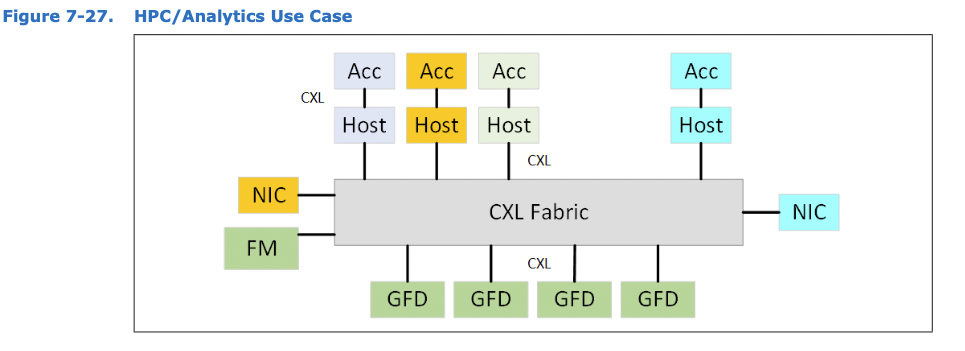
\includegraphics[width=\columnwidth]{figures/hpc-cxl-fabric.pdf}
    % \caption{HPC cores.}
    % \label{fig:hpc-cxl}  
    % }
    % \end{subfigure}
%%%%
    \begin{subfigure}[ht]{0.8\columnwidth}
    \centering{
    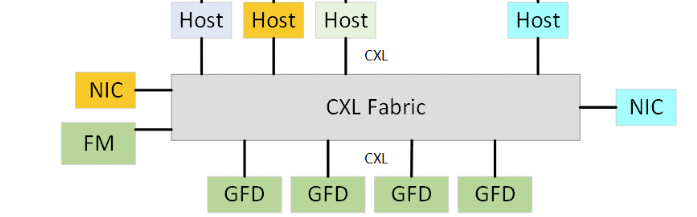
\includegraphics[width=\columnwidth]{./figure/aurelia/kvs-cxl-fabric.pdf}
    \caption{Key-value store for cloud services.}
    \label{fig:kvs-cxl}  
    }
    \end{subfigure}

\caption{CXL fabric abstractive topology.}
\label{fig:cxl-topo}
\end{figure}

\begin{table}[ht!]
\begin{tabular}{|l|l|l|l|}
\hline
            & Bandwidth & Latency & Burstiness         \\ \hline
DL Training & +         & $\triangle$    & -           \\ \hline
HPC         & +         & $\triangle$    & $\triangle$ \\ \hline
KV Store    & -         & +              & +           \\ \hline
\end{tabular}
\caption{Traffic patterns for different workloads.}
\label{tab:cxl-workload}
\end{table}

\section{Challenges}
% \begin{comment}
% list out the challenges related to scalability and latency
% latency     -> congestion control, long stall
% scalability -> routing, coherence traffic monitoring + restriction if possible     
% \end{comment}
%
The current design of CXL fabric~\cite{cxl-3-0-spec} poses challenges on scalability and latency. 
%
First, its addressing and routing design limits the possibility of flexible and dynamic routing. 
%
Second, the lack of an end-to-end transport layer of the fabric makes the fabric prone to congestion and latency spikes. 
%
More importantly, with the usage of load/store instructions, the processor and accelerator that synchronously request data are very sensitive to latency because the latency determines how long they need to stall their execution.
%
The addressing, routing, and transport-level challenges are discussed in the following subsections.  

\subsection{Addressing and Routing Challenges}
\label{sec:motivation:routing}

\noindent \textbf{Routing.}
CXL routes packets with a per-device ID called Port ID on the fabric. 
%
The Port ID-based routing (PBR) addresses each device with a 12-bit ID. 
%
A packet with PBR contains a specific source port ID and destination port ID before it leaves an edge CXL switch that connects directly with devices.
%
Each CXL fabric has a single fabric manager to initialize, bind/unbind devices to ports, and handle event notifications, such as the removal or failure of devices, from the switch.   
%
The fabric manager is equivalent to a centralized software-defined network controller as it controls the per-port forwarding and is aware of all the route changes. 
%
However, CXL fabric has (1) a limiting addressing scheme to support multi-path and adaptive routing, %address devices under multi-level switching
(2) single-path and inactive routing regardless of the traffic condition.

%However, the current CXL routing falls short to achieve its own expectation because of the following reasons.
\noindent \textbf{Challenge: Limited addressing support for multi-path and adaptive routing.}
%
% \stingw{ Yes multi-level routing is feasible with CXL 3.0.
% But SPID and DPID are only used to describe devices.
% The fabric routing is SDN-style, so all routing reconfiguration (with packet sparying or load aware) needs to go through Fabric Manager. This make FM a performance bottleneck.
% }
%
The current PBR routing scheme assigns an ID to devices only. 
%
PBR routes packets to the destination device through multi-level switches with routing installed by the fabric manager. 
%
Any routing reconfiguration needs to go through the fabric manager and thus making load-aware, adaptive routing inefficient and infeasible on a large scale.
%
%PBR with routes controlled by the fabric manager 
The centralized routing of PBR prevents the usage of classic multi-pathing techniques like packet spraying or ECMP because all the routes are pre-determined by the fabric manager.
%
Figure.~\ref{fig:cxl-fabric-overview} shows an example of multi-level CXL fabric.     
%
%if the fabric does not have inter-switch links with a single-level switching.
%
% PBR prevents CXL fabric to realize the multi-level switching that enables a larger topology with switches connected.
%
%PBR cannot route packets through this because it does not address the switches on the fabric.  

\noindent \textbf{Challenge: inflexible routing over diverse topologies.}
CXL fabric supports flexible topology and thus opens the possibility of having a wide range of topologies such as a fully connected graph, Fat-tree~\cite{fat-tree:sigcomm:2008} or Dragonfly~\cite{dragonfly:isca:2008}. 
%
These topologies provide multiple paths for a source and a destination, but CXL fabric cannot route packets over multiple possible paths given its current design.

\subsection{Transport-level Challenges}
\label{sec:motivation:transport}
% The transport of CXL includes PCIe for point-to-point flow control and QoS Telemetry implementing ad hoc rate-throttling for CXL.mem traffic. These two mechanisms are not able to ensure a predictable fabric latency with minimal congestion.  

CXL inherits point-to-point flow control from PCIe that was designed for the communication between the device and CPU rather than a fabric. 
%
The flow control operates between two directly connected endpoints. 
%
They exchange credit tokens to evaluate the available buffer space on each side. 
%

\begin{figure}[t!]  
    \centering
    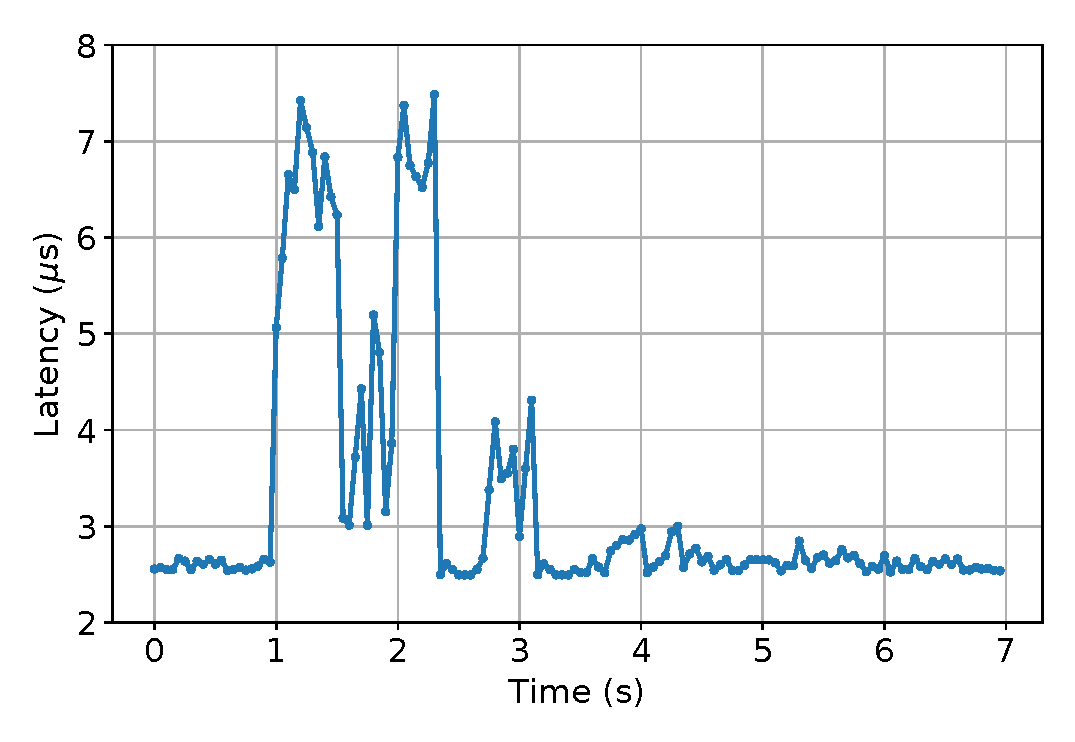
\includegraphics[width=0.8\columnwidth]{figure/aurelia/pcie-congestion.eps}  
    \caption{RDMA latency spikes almost 3 $\times$ by PCIe congestion.}
    \label{fig:pcie-congestion}        
\end{figure}

\noindent \textbf{Challenges: Flow control cannot prevent congestion.}
The point-to-point, credit-based flow control is focused on not overrunning the buffer only. 
%
It cannot deal with pairs of endpoints sharing a port on the switch because no information is exchanged between them. 


\noindent \textbf{PCIe congestion experiment.}
We design an experiment of multiple flows sharing a port on a switch and creating congestion.
%
Given no commercially available hardware for CXL, we use PCIe which shares the same flow control mechanism for our experiment. Interestingly, PCIe congestion has been identified and demonstrated under different setups~\cite{sbfc:ieee-micro:2005, pcie-congestion-model:sc:2016, invisible-probe:oaklnad:2021}. 

We create artificial PCIe congestion on a PCIe switch port shared by two devices. The machine uses a SuperMicro X11SPA-TF motherboard with a Broadcom PEX8747 PCIe switch. The PCIe switch has one upstream port to the CPU, and two downstream ports connecting to the devices, An Nvidia 2080 Ti GPU and a ConnectX-5 RDMA NIC connected to the PCIe switch.
%
\begin{figure}[ht!]  
    \centering
    %includegraphics[width=1\columnwidth, cframe=red!5!red 0.5mm]{figures/pcie-exp.eps}  
    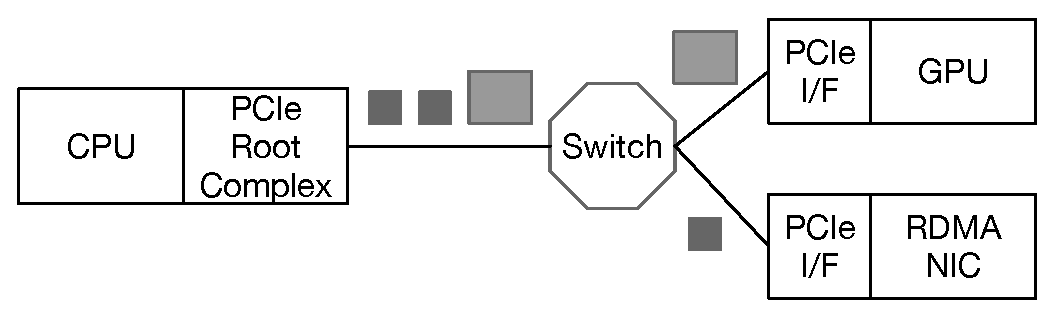
\includegraphics[width=0.8\columnwidth]{figure/aurelia/pcie-exp.eps}  
    %\vspace{-2ex}
    \caption{Experimental setup for PCIe congestion.}
    \label{fig:pcie-experiment}        
\end{figure}
%
The PCIe switch connects with the host processor on one side and provides two ports connecting to GPU and RDMA NIC.
%
The experimental setup is shown in Figure~\ref{fig:pcie-experiment}.
%
During the experiment, the NIC periodically sends RDMA write requests to another machine every 100 microseconds. 
%
Each write request is sent from the CPU and travels through the PCIe switch to the NIC. 
%
After a second, a large integer array of 200 MB is moved from the main memory to the GPU. It causes heavy traffic on the upstream port and the downstream port to the GPU.
%
Their traffic collides on the upstream port of the PCIe switch %as they are both unaware of each other 
because flow control does not consider congestion that is caused by an outgoing link. 

We use PerfTest of Linux-RDMA library to measure the RDMA write request latency~\cite{ofed-perftest} shown in Figure~\ref{fig:pcie-congestion}. The latency spikes to almost 3x from 2.593 $\mu$s to 7.483 $\mu$s at the peak of PCIe congestion. 
%
PCIe's virtual channel is a feasible but not scalable solution because it provides only 7 channels. 
%
Traffic on the same channel still suffers from the same congestion as we have shown above. 
 
%\noindent \textbf{QoS Telemetry insufficiency.}
%QoS telemetry is still insufficient to address all potential congestion issues for the following reasons. 
%
%$First, QoS telemetry is focused on CXL.mem packets. 
%
\noindent \textbf{Challenge: Rate throttling between host CPU and devices only:}
CXL fabric offers a rate throttling mechanism called QoS Telemetry to avoid device overload and possible fabric congestion. 
%
The current QoS telemetry is designed specifically for CXL.mem between the host and devices with its local memory.
%
QoS telemetry allows memory devices to indicate their current internal load with 2 bits for CXL.mem response packets.  
%
The sender on the host CPU uses the reported internal load to monitor and throttle its request rate. 
%
However, not every sender on CXL fabric is on the host CPU. 
%
Peer-to-peer memory accesses using Unordered I/O in CXL.io support devices accessing the memory of another device directly. 
%
These peer-to-peer accesses under CXL.io are not throttled in the current design because QoS telemetry is only for CXL.mem and does not consider the sender to be other than a host CPU.
%
Machine learning and HPC applications illustrated in Figure~\ref{fig:cxl-topo} have evolved into heavy use of accelerators. 
Overlooking memory access from devices, especially accelerators, limits CXL fabric's ability to mitigate congestion and device overload.

%The rate throttling targets specifically for devices, mainly memory devices, that are associated with a host in the current design. 

%
% Perform rate throttling on CXL.mem packets alone cannot mitigate possible congestion because packets using the other protocols share the fabric.
%
%It is used for devices with its local memory including memory expansion devices and accelerators with device memory, e.g. GPU, FPGA, and ASIC.


%\TODO{merge this one with rate throttling}
%\noindent \textbf{Limit usage of load & congestion information}
%
%QoS telemetry does not consider peer-to-peer memory access packets on CXL.io protocols just introduced in the CXL 3.0 specification.
%

% \noindent \textbf{Challenge: Host controlled rate throttling}
% The request throttling of QoS telemetry is designed to be operated by the host.
% %
% It does not consider memory access can be initiated from devices, especially in a peer-to-peer fashion. 
% %
% These devices contain logic for a specific workload but do not have any general-purpose cores attached.
% %
% The current QoS telemetry design does not allow these accelerators to throttle themselves according to the device load. 
% %
% \stingw{I think we can still leave the rate throttling on host but it needs to be efficient like polling?}
% Moreover, a device performing peer-to-peer memory access depends on the host to throttle its request rate. 
% %
% %This contradicts the promise of resource disggreattion on a CXL fabric.
% This adds additional latency for throttling and thus risking more congestion on the fabric. 
%\stingw{we'll need additional hardware logic on CXL device that will initiate memory request}

\noindent \textbf{Challenge: Inaccurate load \& congestion information.}
QoS telemetry devises a mechanism called Egress Port Backpressure (EP Backpressure) to indicate the load of CXL switch ports.
%
It monitors the flow control backpressure situation on each CXL switch egress port. 
%
If the port cannot transmit packets due to insufficient credits, the port marks a 2-bit EP Backpressure value on the device load field of the outgoing request. 
% Omit the Temporary Throughput Reduction here
%
The overall load of a device is determined by the maxima of the device's internal load and EP Backpressure. 

However, the overall device load subsumes EP Backpressure, which is valuable congestion information. 
%
By taking the max value of the separated piece of information, QoS telemetry provides neither accurate device internal load nor congestion on the fabric.
%
The inaccurate information prevents QoS telemetry from performing end-to-end flow control and congestion control for the transport protocol.
%
The aforementioned challenges motivate us to design \aurelia. 
%
%\TODO{find place to say switch and CXL device are both nodes on a CXL}
\section{Design of \aurelia}
\label{sec:design}
% \stingw{Reduce specific details on routing, merge multi-path and alternative routing. the design rationale is more important. we don't want to be tied to a 
% specific solution or design point.}

\begin{figure}[t!]    
    \centering
    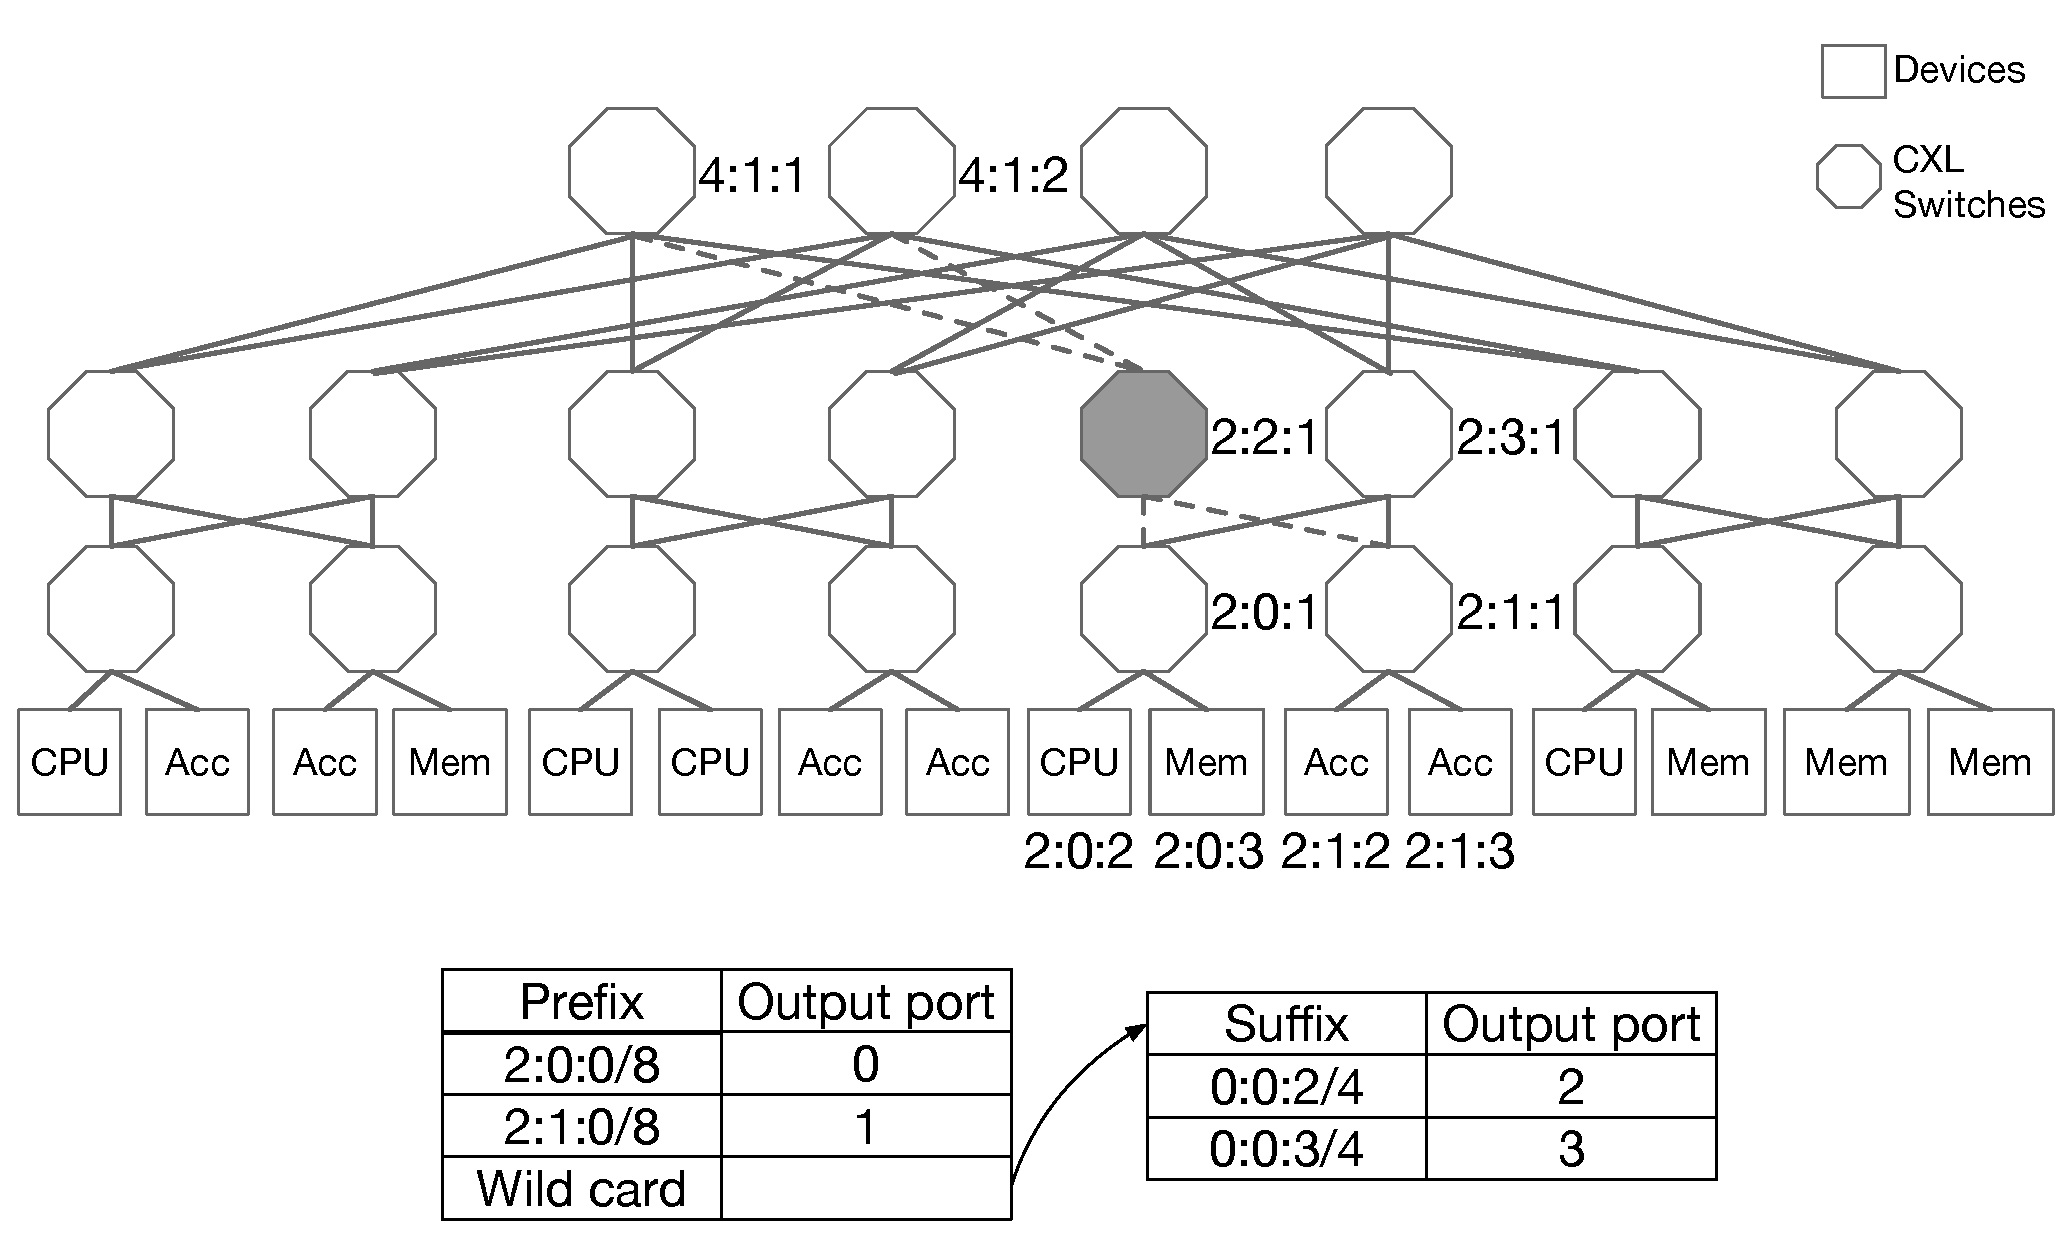
\includegraphics[width=0.9\columnwidth]{figure/aurelia/cxl-fat-tree-routing-table.eps}
    \caption{CXL fabric as a Fat-tree using 12-bit FAN-ID address \emph{X:Y:Z}, which X, Y, and Z are hexadecimal values. Dash lines represent the routes from switch \emph{2:2:1}'s routing table.} 
    %representing \emph{pod:switch:device}}
    \label{fig:cxl-fabric-overview}
\end{figure}

We propose \aurelia, a network design involving devices and switches on CXL fabric. \aurelia provides addressing, routing, and congestion control protocol design by augmenting necessary functionalities on the fabric interface and switches.

\subsection{Addressing \& Flow}
%
\aurelia proposes to generalize CXL's port ID scheme to assign a 12-bit fabric node ID (FAN-ID) to a node that is either a device or a switch on the fabric. 
%
This is analogous to the 32-bit IP address describing hosts in an IP network.
%
%
FAN-ID assignment is agnostic to the underlying topology as long as a FAN-ID is unique for a node on a CXL fabric. 
%
Currently, \aurelia assigns FAN-ID to the physical interface of the device. It does not assign FAN-ID to logical interfaces sharing the same physical interface.
%
%\aurelia considers multi-tenancy a device-specific detail and do not provide additional FAN-ID to logical CXL interfaces
%Multi-tenancy of devices is out of the scope of this work.


With a similar analogy of "5-tuple" in the IP network, \aurelia defines a flow by a sequence of CXL packets that shares the same source device, destination device, protocol, and message classes.
%
Thus, routable CXL packets can be identified with a quadruple: \emph{(Source FAN-ID, Destination FAN-ID, CXL protocol, message classes)}. The CXL protocols include CXL.io, CXL.mem, and CXL.cache. The message classes are sub-type of packets within each protocol. For example, a CXL.mem packet writing to a device belongs to a class of \emph{M2S Request with Data} and a CXL.cache packet that carries responses from the device to the host belongs to a class of \emph{D2H Response with Data}.
%
Fat-tree with oversubscription is out of the scope of this preliminary study. 
%
For the rest of \aurelia's design, non-oversubscribed Fat-tree is assumed as the underlying topology. Different topology constructions and options are discussed in Sec.~\ref{sec:discussion}.
%

% \begin{comment}
% %FAN-ID 
% %because routing design can be based on per-node FAN-ID
% %each device usually has a single CXL interface with potentially different number of lanes. 

% Also, given the limit size of 12-bit address space, it is not efficient to assign multiple addressses to a single switch. 

% Per port address design like MAC address is not necessary
% because \aurelia's routing design is modeled after IP level routing on switches. 

% dragonfly's routing
% Minimal (MIN) : The minimal path is taken as described in
% Section 4.1.
% Valiant (VAL) [32] : Randomized non-minimal routing as
% described in Section 4.1.
% Universal Globally-Adaptive Load-balanced [29] (UGALG, UGAL-L) UGAL chooses between MIN and VAL on a
% packet-by-packet basis to load-balance the network. The
% choice is made by using queue length and hop count to estimate network delay and choosing the path with minimum
% delay. We implement two versions of UGAL.
% UGAL-L – uses local queue information at the current
% router node
% \end{comment}

% \begin{figure}[htb]
%     \centering
%     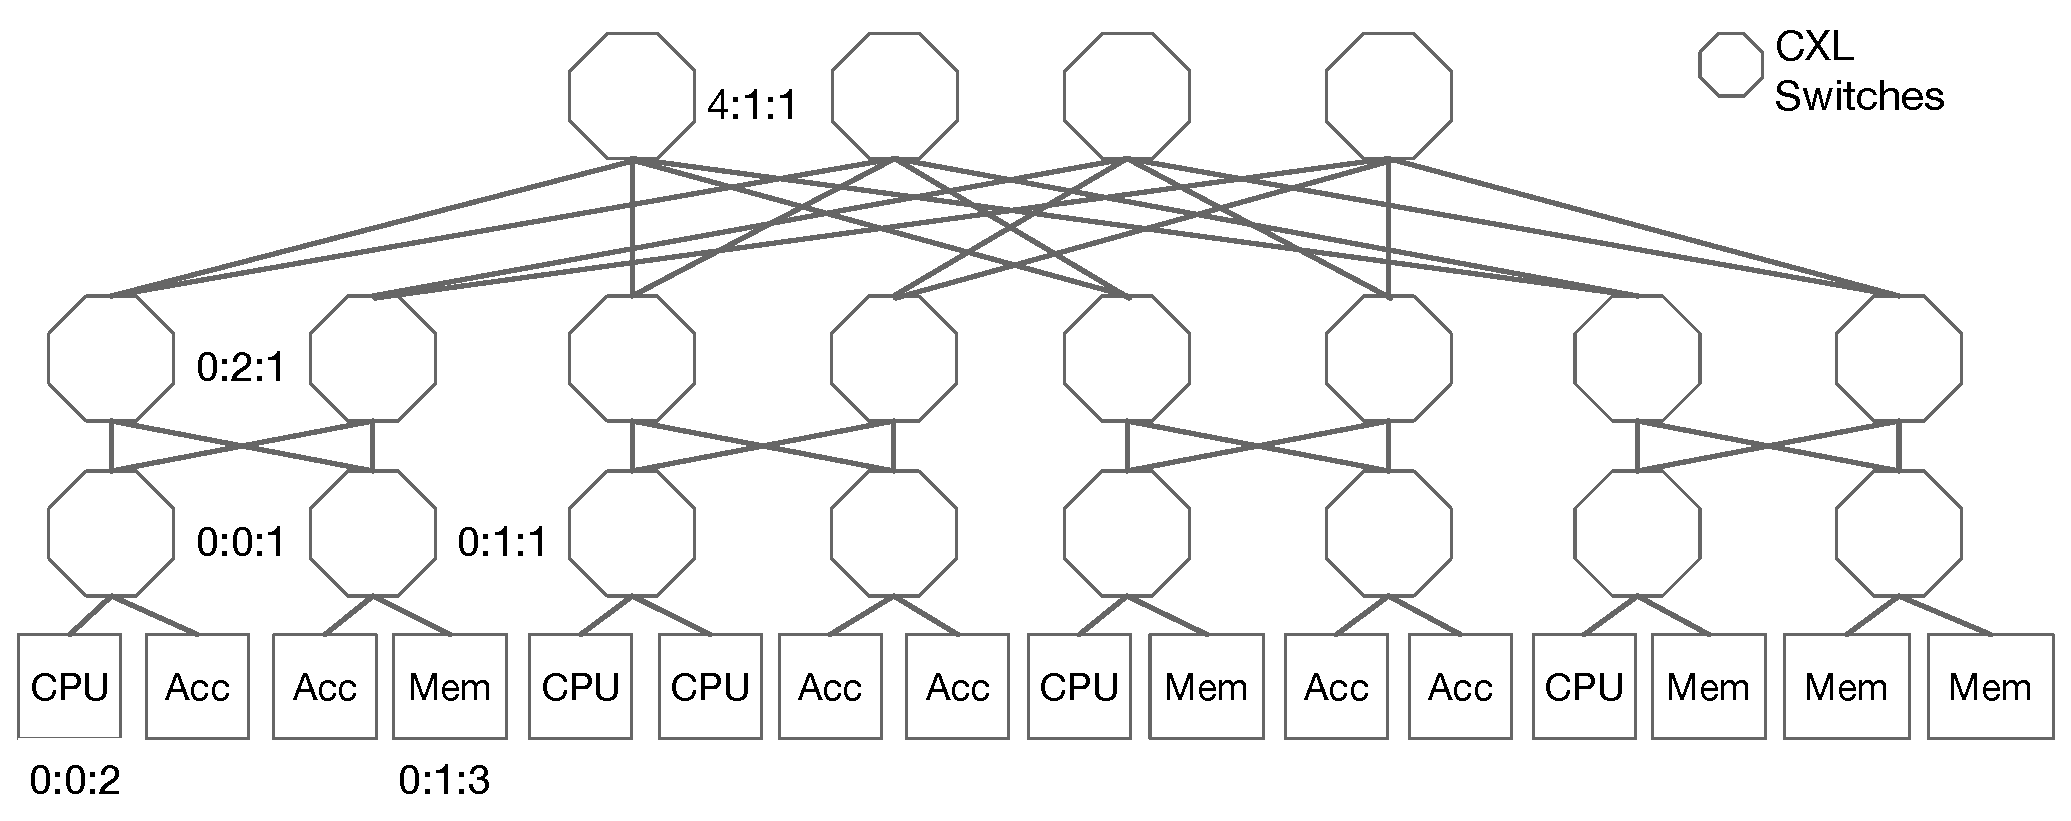
\includegraphics[width=\columnwidth]{figures/cxl-fat-tree-clear.eps}
%     \caption{\TODO{Routing example on Fat-tree.}} %representing \emph{pod:switch:device}}
%     \label{fig:fat-tree-routing}
% \end{figure}

\subsection{Routing}
% P Path selection, R Routing itself, and L Load balancing. 
% Path selection determines which paths can be used for sending a given packet. Routing itself
% Routing answers a question on how the packet finds a way to its destination.
% Load balancing determines which path (out of identified alternatives) should be used for sending a packet to maximize performance and minimize congestion.

\aurelia routes packets based on FAN-ID addresses like IP routing.
%
CXL switches route a packet based on its routing table that maps a group of FAN-ID destinations onto a port. 
%
CXL switches transmit the packet out of a specific port to another switch that knows the next hop of this packet. 
%
The forwarding keeps on until the packet reaches the FAN-ID destination.

\noindent \textbf{Routing: Fat-tree as an example.}
%
Constructing a Fat-tree~\cite{fat-tree:sigcomm:2008} with 12-bit FAN-ID address shows a $k$-ary fat-tree with $k=4$ in Figure~\ref{fig:cxl-fabric-overview}.
%
Fat-tree uses a hierarchical scheme that assigns FAN-ID to nodes as \emph{pod:switch:device} with three segments.
%
Each segment is a 4-bit exact, hexadecimal value.  
%
For example, the leftmost CPU has FAN-ID \emph{2:0:2} representing it belongs to the third pod, the first switch, and the third node which is right after the switch itself.
%
Like IP routing, the routing on Fat-tree takes a single shortest path despite that the Fat-tree topology provides path diversity.
%
This creates bottlenecks even for trivial communication patterns because of the underutilization of available bandwidth.
%
Fat-tree implements a two-level routing table on each switch. One level of the table routes traffic down to the device and another one routes traffic toward the core of the fabric.
%
The table maps a set of destinations to a specific port. The routing lookup of destinations uses the address prefix for the traffic downward to the devices and the address suffix for the traffic going toward the cores.
%
The address suffix approach spreads traffic toward the fat-tree core across different switches based on FAN-ID.
%
The bottom of Figure~\ref{fig:cxl-fabric-overview} shows the routing table of CXL switch \emph{2:2:1} filled in gray. The prefix table routes packets toward its downstream switches \emph{2:0:1} and \emph{2:1:1}. The suffix table routes the packet upward to core switches \emph{4:1:1} and \emph{4:1:2}.  
%\TODO{add a running example on to Figure~\ref{fig:fat-tree-routing} or a new one.}


\noindent \textbf{Multi-path routing.}
%
The two-level routing table of Fat-tree is just an implementation of multi-path routing together with a specific topology. \aurelia imposes no restriction on how the fabric should be constructed. Instead, \aurelia requires routing tables to be able to map a destination to multiple next-hop FAN-ID and its corresponding metric. The metric can be distances in terms of hops or local congestion level on each switch port. 
%
\aurelia selects a next-hop with minimal metric and randomly selects one if there are multiple next-hop options with equal metric.  
%
Considering the number of hops for shortest path routing, \aurelia can perform a random selection for the next hop on flow granularity or on packet granularity. The former is similar to Equal-Cost Multipathing (ECMP) and the latter is similar to packet spraying. 
%

% \begin{comment}
% After identifying the quadruple, the existing knowledge of using flow as a major abstraction of load balancing and optimization becomes applicable for CXL fabric flow~\cite{FlowBender, Hedera, MicroTE}. In the case of multi-tenant devices, the quadruple cannot distinguish traffic between different tenants. Thus, per-packet load balancing schemes are more applicable for multi-tenant scenarios~\cite{Fastpass, DeTail, MPTCP}. 

% \weitao{Since we already assume next-generation connection, do we want to mention that the fat-tree topology can be a baseline, and we could further optimize the topology based on the application traffic pattern, like adding more number of lanes between frequently communicated devices.} 
% \stingw{I agree. topological optimization is a nice direction but it's hard to do it with current or near-future CXL technology. We can put it to the Discussion.}
% \stingw{We'll need CXL with higher radix to have more exotic topology, e.g. Dragonfly, Jellyfish, Xpander}

% \weitao{Active routing is another interesting type of routing. It is developed based on load-balancing routing. When one path is congested for a substantial amount of time, some flows will change the flow label to change the 5-tuple, so that the flow will pick a new path automatically. In your case, do you think you can also add a similar thing in "5-tuple" to make it "6-tuple" and enable active routing?} \stingw{introducing additional things on CXL's 256-byte packet is hard given the limited space. I don't agree with this one.}
% \end{comment}

% \TODO{we should talk about how the fabric manager will be implemented. GPU-SSD example is not a good one.}
% \reviwer{B: I encourage you to be more explicit about what's in/out of scope for the fabric manager}
\noindent \textbf{Adaptive routing.}
%
ECMP and packet spraying are oblivious to the workload. 
%
\aurelia can further exploit local per-port information on the switches or the fabric manager manipulating the routing table to achieve adaptive routing.
%
\aurelia uses per-port EP Backpressure as a measure of local congestion indication. 
%
For selecting an egress port with minimal congestion on the switch, \aurelia uses power-of-2 choice~\cite{power-of-two:tpds:2001} to avoid congestion on ports based on possibly delayed congestion information.
%
Additionally, \aurelia allows the fabric manager to insert routes and has the sole authority to modify the routing table at any time.
%
This is useful for the workload that requires non-trivial routes tailored to specific workloads~\cite{gullfoss:tech-report:2015, fractos:eurosys:2022}. 
%mirador:fast:2017, 
%uses multiple devices together~\cite{gullfoss:tech-report:2015, fractos:eurosys:2022}.
%
% \stingw{take out the GPU example!}
% The GPU-SSD example in Sec~\ref{sec:motivation:routing} is exactly one of these workloads.
% %
% The detouring of peer-to-peer memory access to an additional hop of memory buffer is not trivial to be specified as routing rules. 
% %
% The fabric manager first determines a fabric-attached memory device as the destination, then redirect the routing between the producer and the consumer devices to the memory device instead.  
% %
% The fabric manager then asks the consumer to read from the specific memory device instead of directly communicating with the producer.

\begin{figure}[ht!]
    \centering
    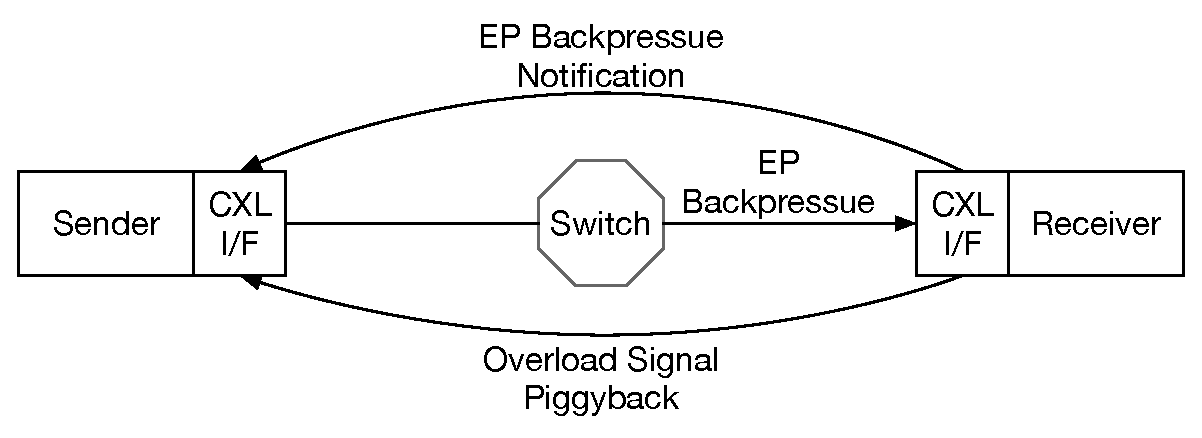
\includegraphics[width=0.9\columnwidth]{figure/aurelia/congestion-control-flow.eps}
    \caption{\aurelia has a congestion control loop for the fabric, a flow-control loop for the device.}
    \label{fig:congestion-control}
\end{figure}

\subsection{End-to-end Congestion Control}
% \stingw{More on pointing out the unique challenge, don't argue against delay based approach too much. Stay neutral before we have strong evidence.}
% \balance
% \begin{comment}
% These devices have shallow buffer space and different rate of producing/consuming data. %and are allocated with different bandwidth on the fabric.
% %
% With strictly peer-to-peer communication, the producer matches consumer's rate to not overwhelm the consumer. 
% %
% The slow-down on faster producer leads to under-utilization of the device. 
% %
% To improve resource utilization, fabric attached memory pool can serve as the buffer and an alternative routing destination between devices. 
% %
% This decouples the producer and the consumer and allows faster producer to be utilized by other workload.
% %
% The switch identifies CXL.io packets performing peer-to-peer memory access, and notifies the fabric manager when it sees EP Backpressure on its port with CXL.io.
% %
% The fabric manager modifies the routing table between the producer and consumer, and routes the packets to a specific fabric attached memory pool attached to the either side of the CXL switch. 
% %
% The fabric manager then asks the consumer to read from the specific fabric attached memory pool instead of directly communicating with the producer.

% \weitao{One suggestion about the signals: the internal load and the EP backpressure could be represented in a uniform format. Both of them suggest the congestion level, but for end-point devices and switches respectively.}\stingw{this sounds about right!}

% \weitao{Another wild idea is that, if switches and end-point devices could provide more quantitative signals (like 8 bits) to represent congestion level, rather than a single bit to provide a binary signal about congestion, the performance of the congestion control algorithms could be largely improved. As a supporting fact, many commodity switches can support reporting and piggybacking telemetry information for each packet, including per-hop queueing delay and per-hop utilization.}\stingw{the problem with CXL is the packet is 256-byte. we could argue for using more bits in the discussion section. I tried to do the minimal modification to CXL to achieve something useful.}    
% \end{comment}

\aurelia implements end-to-end congestion control with overload avoidance by extending existing mechanisms of CXL. 
%
The existing mechanisms are EP Backpressure, rate throttling, and internal load reported by devices.
%
EP Backpressure describes the queuing situation in a similar way as Explicit Congestion Notification (ECN) does on Ethernet and Infiniband.
%
EP Backpressure and ECN both indicate congestion explicitly to the receiving endpoints and need packets to convoy the congestion signal back to the sender.
%
Rate throttling controls the data injection rate into the fabric and thus avoids congestion. 
%
%On top of these mechanisms, CXL fabric is a lossless fabric by its point-to-point flow control design.
%
Internal load is used to avoid overloading device that is likely to cause additional device-side delay or loss of CXL packets.
%
These factors determine \aurelia to implement a rate-based congestion control with overload avoidance for the devices. 


\aurelia separates EP Backpressure and the device's internal load for congestion control and overload avoidance.
%as two different metrics as they represent device and fabric information.
%
EP Backpressure as a 2-bit congestion signal on the fabric is piggybacked to the sender if its value is larger than a threshold.
%
The 2-bit device internal load serves a quantized credit for the sender not exceeding the receiver's processing rate.
%
Using credit to regulate sending rate effectively achieves end-to-end flow control to avoid overloading. 
%
Flow control preventing buffer-overrun is handled by the link and physical layer of CXL and thus not a concern for the transport layer. 
%
Also, \aurelia generalizes the reporting of device internal load for all memory access, including peer-to-peer memory access between devices.

Peer-to-peer memory access between devices without embedded CPU motivates the need of implementing rate throttling logic on CXL interface hardware.   
%
Also, rate throttling has a tight latency requirement of sub-$\mu$s on CXL fabric.
%
Pond measured end-to-end CXL.mem latency and obtained latency ranging to 270 ns on CXL system with a single switch~\cite{cxl:hoti:2022, pond:asplos:2023}. Using Pond's latency assumption, the latency of CXL packet traveling through a two-level fat-tree takes around 680 ns.


Combining sub-$\mu$s latency and peer-to-peer memory access requirements, \aurelia relies on hardware to throttle rate for congestion control. 
%
The configuration of these hardware is kept on the host CPU, but the actual rate throttling is on hardware to meet these requirements.  
%
Implementing rate throttling logic on hardware has been used on RDMA over Infiniband and Ethernet with RoCEv2 support.
%
Hardware-based rate throttling ensures all devices on the CXL fabric are able to control their injection rate and further regulate the congestion.   
%
Before throttling, \aurelia sets the rate as the target rate for later recovery.
%
\aurelia throttles the rate of the sender, when the receiver notifies it of the congestion signal and generates EP Backpressure. 
%
After rate throttling, \aurelia enters the recovery phase and then performs additive increase when approaching the target rate~\cite{dcqcn:sigcomm:2015}.   



%%
% Congestion control on existing lossless fabric, such as Infiniband, DCQCN for RoCEv2, implemented a rate-based congestion control algorithm requireing Explicit Congestion Notification (ECN) on switch to indicate congestion.
%
% Infiniband switches mark packets with a Forward ECN (FECN) bit when congestion is detected~\cite{infiniband-spec}. 
% %
% The destination node receives the FECN-marked packets and sends a Backward ECN (BECN) marked packet to the source node.
% % 
% The source node throttles its injection rate when it gets packets with BECN. The throttling over time reduces congestion and the fabric returns to a state without any congestion. 
% %
% Thee FECN marking of packets requires switch support and the implementation of BECN and rate throttling requires additional logic in CXL interface hardware.
%
% DCQCN, a congestion control protocol designed for RoCEv2, relies on the ECN of Ethernet to notify the source so the the source adjusts their injection rate similar to Infiniband~\cite{dcqcn:sigcomm:2015}.

% Another category of congestion control protocols is based on delay~\cite{timely:sigcomm:2015, swift:sigcomm:2020}. They make sense on Ethernet/IP networks because NICs are equipped with hardware timestamping. 
% %
% Also, the PTP protocol enables high-precision time synchronization over the network. 
% %
% Both of these requirements are infeasible for the CXL interface. 
% %
% First, measuring accurate delay requires every CXL interface to support hardware timestamping.
% %
% Second, PTP time synchronization does not run over CXL protocol and it needs a high-precision time source on every instance of CXL fabric. 
% %
% These two requirements add expensive costs to hardware and thus make it infeasible.  

% \aurelia implements a transport layer with rate-based congestion control with hardware-based rate throttling, and ECN-like usage of EP Backpressure.
%



%1. rate throttling 
%
% This sub-$\mu$s latnecy makes rate throttling hard on host CPU because state-of-the-art low-latency networking stacks on CPU react in 5 or more $\mu$s~\cite{shenango:nsdi:2019, shinjuku:nsdi:2019, caladan:osdi:2020}. The $\mu$s-level reaction time makes them only possible to be used as a fallback option.

%
% As EP Backpressure sets the device load on the request packet, the destination sends a memory response with devload indicating the port congestion alone. This response is not a piggyback like the device reporting the internal load. This egress port backpressure notification should trigger rate throttling on the source side (which can be a host or an autonomous device).    
% \stingw{we should be more specific about the term memory request and response}.   

%
% Previous study of congestion control on lossless fabric, such as Infiniband, DCQCN for RoCEv2, follows a very similar approach.  
% Both of them implemented a rate based congestion control algorithm in hardware and requires Explicit Congestion Notification (ECN) on switch to indicate congestion. 
%
%To prevent packet loss, Infiniband implements credit based flow control on its link layer and RoCEv2 implements PFC on Ethernet. 
%
% Infiniband switches mark packets with a Forward ECN (FECN) bit when congestion is detected. 
% %
% The destination node gets the packets with FECN-marked and sends the source node a packet marked with Backward ECN (BECN) bit.
% % 
% The source node throttles its injection rate when it gets packets with BECN. The throttling over time reduces congestion and the fabric returns to a state without any congestion. 
% %
% Thee FECN marking of packets requires switch support and the implementation of BECN and rate throttling requires additional logic in CXL hardware interface IP.
% %
% DCQCN, a congestion control protocol designed for RoCEv2, relies on ECN of Ethernet to notify the source node so the the source node could adjust their injection rate in a similar manner as Infiniband.



%\subsection{Programmability: Active Networking revisit}

%\TODO{what's active network and what does it matter to CXL}
%Outline of the design 
% \begin{itemize}
% \item Making CXL a proper network, adding L3 and L4
% \item If we have a system with the refined CXL fabrics with proper L3 and L4, then what kind of abstraction should we use to program this kind of disaggregated system? -> active network
% \end{itemize}
% \stingw{Topology-aware congest:}
%\noindent \textbf{Overview:}

%--------------------------%--------------------------%--------------------------%--------------------------%--------------------------%
%
% Also, these devices usually have limited buffer space to store incoming data from the fabric. 
% %
% Shallow buffer has smaller headroom to absorb bursts of data before pausing and congesting the link
% %
% This motivates exploring multiple paths to route around links with lower bandwidth or other undesirable property. 

% how routing can take congestion and multi-path into consideration.
% \stingw{Topology-aware multi-path routing:}
% -> Multiple paths can be found on Dragonfly in ~\cite{aquila:nsdi:2022} and some other HPC used topology.
% -> From the datacenter literature, ECMP spraying packet to alleviate possible congestion on Clos based topology. (indirect topology)
% -> Dragonfly topology with more direct node-to-node links. 

% What's the difference and shortcoming of CXL fabrics compared to exitsing network?
% 1. CXL fabric is different from the current network like Ethernet or Infiniband as its end points/pass-through points are devices may have none to little power of general purpose compute. The entire stack of this network is hardware based. The congestion control algorithm needs to be implemented with little hardware addition on top of PCIe.
% 2. CPU is still needed here but it does not need to be an endpoint but for setting up/tearing down the flow.

% After establishing CXL after refinement could be a good network, we should argue about how we should program it. we should consider active network.
% \begin{itemize}
% \item why are we using active network as the inspiration? Active network has the idea of embedding compute into the fabric if the compute is better to be performed on the fabric rather than on end-host CPU.
% \item Accelerator and device as the major residents on the fabric instead of a large amount of powerful general-purpose CPU cores.
% \item Accelerator and device like network switches are programmable but not general-purpose. They don't have the control structure to hold or terminate a flow or connection in anyway.
% \item We want an abstraction capturing data movement and related compute with it.
% \item If we want to implement ActiveCXL, what are the missing pieces from CXL spec and current supported hardware?
% \item $\rightarrow$
% (1) flow as an abstraction for applications to reason about,
% (2) capability as a way for distributed control flow?
% (3) Discrete switch style to load large program on accelerators and capsule style for smaller programs and loaded large programs,
% (4) packet framing on top of CXL packets for meaningful execution,
% (5) capsules for data transformation and loaded kernels on accelerators,
% (6) CPU cores still hold the control information for the setup and tear-down of the flows but they are completely off the data path to avoid becoming bottlenecks.
% \end{itemize}

% CXL presents a lossless fabric with its point-to-point flow control. 
% %
% CXL requires a hardware implementation as devices do not always have general purpose CPU core to run the congestion control algorithm. 
% %
% Some of CXL devices do not have the ability to determine its injection rate as they are directed by the CPU as a subordinate.
% %
% Also, CXL interface has small buffer to store its  


%
% \stingw{dragonfly just leave it in the discussion, saying we need higher radix}
% Path diversity!
% \stingw{first, ECMP}
% On the inter-switch level:
% \stingw{topological specific solution -> ECMP if in the case of Clos}
% "An equal-cost multipath (ECMP) set is formed when the routing table contains multiple next-hop addresses for the same destination with equal cost. (Routes of equal cost have the same preference and metric values.) If there is an ECMP set for the active route, Junos OS uses a hash algorithm to choose one of the next-hop addresses in the ECMP set to install in the forwarding table."

%"The PBR Edge request port shall decode the request HPA to determine the DPID of the target GFD, using the Fabric Address Segment Table (FAST) and the Interleave DPID Table (IDT)"

% end-to-end level consideration
% Explain the control plane overhead: 
% 1. storing more routes on the switch -> maintain a cache and swap the route in when it's not available
% 2. The routes are only needed to be re-populated when switch failure or device removal on a fabric manager
% 3. maintain link congestion level in a table when multiple routes are presented 
% %
% explain data plane overhead:
% 1. lookup queuing situation on outgoing inter-switch links
% %
% Usually the fabric manager populates the routes in a SDN-style.
% in the case of performance reroute, device   
% (1) switch maintains additional fabric based memory buffer as alternative destination 
% (2) when reroute happens, 
% slow path: switch notify the fabric manager, the fabric manager asks the destination to pull/read from the fabric buffer

%\stingw{how do we use rate throttling?}
% \stingw{define autonomous device somewhere earlier?}
% Rate throttling ideally will be implemented as hardware on CXL interface for "autonomous" devices that are able to initiate CXL requests.
% Compared to solely doing on host, this improves the control responsiveness and make these device autonomous.  


\section{Evaluation of \aurelia's Design}
\label{sec:cc-design}
%
We simulate the design of \aurelia because CXL hardware supporting CXL fabric is not available to the author at the time of writing.
% 
The simulation setup and parameters are cross-checked with public available reports~\cite{pond:asplos:2023, demystifying-cxl:micro:2023,h3platform-cxl-memory}. 
%
Our reported numbers are calibrated with H3 platform's CXL memory expansion chassis~\cite{h3platform-cxl-memory}. The difference between our simulation and the reported numbers are within 5\%.

\subsection{Packet-level Simulation with ns-3}
We use NS3~\cite{ns-3} to simulate packet level behavior on a CXL fabric.
%  
NS3 is a discrete-event network simulator that is open-sourced and well-established in the research community. 
%
Previous implementations of lossless fabric using ns-3 are focused on RDMA over Converged Ethernet (RoCE)~\cite{dcqcn:sigcomm:2015, hpcc:sigcomm:2019,pint:sigcomm:2020}.
%
These implementations are not usable for CXL fabrics. 
%
They assume the usage of Ethernet, IP, and the RDMA interface cards.
%
CXL fabrics assumes none of those as the devices on the fabric issue load/store instructions directly.  
%  
Our implementation uses the primitive, built-in NS3 classes and starts from scratch. 
%
It simulates CXL's transaction layer and link layer in 256B filt mode.
%
This assumes an underlying PCIe 6.0 physical layer with its forward error correction are fully controlled by the hardware.     
%
All channels of CXL.mem and CXL.cache are supported.
%
\stingw{Maybe we need more description of CXL layers}
Packing of CXL.mem and CXL.cache messages are implemented to ensure the number of packets on the fabric are accurate.  
%
CXL.io functionalities are partially supported as needed.       
%
It enables multi-level switching by extending CXL's port-based routing with~\aurelia's additional mechanism.  

\subsection{Simulation Results on YCSB Benchmarks}
\TODO{CC results with ns-3 simulation}

%\section{Additional Fabric Enhancement Consideration}
\section{Discussion}
\label{sec:discussion}
%\TODO{extending discussion for 6-page HotNets}
% \noindent \textbf{The scale and economic of CXL fabric}
% how large should we scale CXL fabric to be still cost-effective~\cite{pond:asplos:2023}?
% Pond dem
\noindent \textbf{Alternatives: NVLink and PCIe fabric.}
%\TODO{Clean up the text here!}
% \stingw{Here to add NVLink + GH-200 discussion. 
% NVLink is propriety and has a narrower usage even with GH-200.
% GH-200 with NVLink is at most a CXL type-2 usage.
% }
%\stingw{All these alternatives are not designed to be as general as CXL}
%
% Alternative interconnects are designed for specific use cases, and they lack of the generality of CXL. 
% 
NVLink is an interconnect by Nvidia for high throughput between GPUs~\cite{nvlink}. NVLink supports GPU-CPU interconnect with cache coherency on the recent Grace-Hopper 200 hardware~\cite{dgx-gh200}. 
%
NVLink presents an interesting alternative to CXL but has three limitations. 
%
First, NVLink with its cache coherent extension in fact supports GPUs as CXL type 2 devices. However, it does not support CXL type 3 devices that expand memory independent of the main memory capacity. The capability to scale memory capacity is attractive for memory-hungry large language models~\cite{gpt3:neurips:2020,llama:arxiv:2023}. 
%%NVLink with its cache coherent extension presents an alternative of CXL Type2 interconnect.   
%
Second, NVLink scales to 256 endpoints though connects only GPUs as endpoints~\cite{dgx-superpod}. 
%\stingw{Third, NVLink itself does not scale beyond 8 or 16 GPUs on a server.}
Third, NVLink as a propriety interconnect limits its usage beyond Nvidia's hardware.
%
PCIe using Non-Transparent Bridge (NTB) expands beyond a single root complex to multiple hosts as a fabric with many more connected devices~\cite{pcie-spec}. 
%
%PCIe transactions mapped to NTB’s specific memory range are forwarded
%with address translation to the destination host.   
%
% Using NTB with a shared address space spanning all hosts and their devices enables devices to directly communicate with point-to-point DMA over PCIe fabric~\cite{gigaio-fabrex}.
%
However, PCIe, included in CXL as CXL.io, lacks the memory and caching semantics that are much needed in the face of accelerator and memory expansion. 
%
This is exactly the reason that motivates the creation of CXL.
%
Both NVLink and PCIe fabric show a fabric supporting a subset of CXL's use cases but not all of it.    
%
%\stingw{why not hooking Ethernet directly to each device?}

\noindent \textbf{Co-existence of CXL and Ethernet.}
Given the scaling discussion, CXL is still unlikely to completely replace Ethernet in the datacenter due to its current PCIe based physical layer design. 
%
We speculate CXL fabric is beneficial on rack-scale because of the signal integrity and CXL switch hardware cost. 
%
CXL fabric is not intended to replace existing Ethernet completely but as a cost-effective alternative on the rack level. 
%
CXL packets are converted to Ethernet frames at a location equivalent to a top-of-rack switch for cross-rack traffic.
%
Previous work investigating the co-existence of Ethernet and a memory fabric follows a similar approach~\cite{aquila:nsdi:2022}.

%\stingw{Interconnect comparison: NVLink + C2C, other inter core interconnect, PCIe, CXL}
\noindent \textbf{Cost-effective scales of CXL fabric:}
%\noindent \textbf{Co-existence of CXL and Ethernet.}
% \stingw{how large should we scale CXL fabric to be still cost-effective~\cite{pond:asplos:2023}?}
%
CXL is an exciting technology but it comes with its limitations.
%
First, CXL requires retimer to maintain its signal integrity after 500 mm distance~\cite{microchip-cxl-retimer,asteralabs-pcie-retimer}. The retimer raises the hardware cost and incurs extra 20 ns latency every 500 ~\cite{pond:asplos:2023}.
%
Second, to scale CXL supporting multi-level switching, multiple CXL switches are used. They cause an estimated 70 ns latency for each hop over a switch.
%
Considering the combined cost of switches, retimers and additional memory controllers, Pond~\cite{pond-saving:ieee-micro:2023} suggests a
scale smaller than 32-socket for their memory expansion usage (Shown in Figure~\ref{fig:kvs-cxl}).
%
However, the exact scale of cost-effective CXL fabric for model training and HPC usage (Shown in Figure~\ref{fig:ml-acc-cxl}) remains to be determined in future works. 
%
%Pond also suggests the exact scale of a cost-effective CXL fabric depends highly on the workload, e.g. Pond's memory expansion usage for VM on public cloud.

% \stingw{CXL is not a solution for everything. It has signal integrity limits that making it scale beyond not cost-effective and with bloated latency by these intermediate retimers and switches.}
%
% \stingw{Pond suggest 8-socket for the use case is shown as Figure 1-(b). Pond also said that the exact scale depends on the workload. If the workload can tolerate higher latency or has a clear and predictable memory access pattern, then the scale of CXL can be larger if it's cost-effective.}
%    

\noindent \textbf{Topologies and multipathing.}
The flexible topology of CXL fabric empowers the fabric operator to optimize their topology based on the traffic pattern. 
%
The to-be-released CXL 3.1 will support native multipathing. Topologies with high path diversity such as Dragonfly can be easily implemented with CXL's multipathing. 
%
Packet spraying and ECMP on Fat-tree related topologies can be benefited from this as well.
%
With CXL switch prototype supporting 32-port ~\cite{xconn-cxl2-switch}, we expect these higher radix switches to enable us to explore different design options.
%
For example, the fabric operator can assign a high over-subscription ratio if the traffic pattern demonstrates high localities under a CXL switch. 
%
As another example, the fabric operator can add or reduce the bandwidth of certain CXL to better match the bandwidth to the actual demand between particular nodes. 

\noindent \textbf{Security implication: Delay based side channel.}
CXL fabric exposes the server interconnect to a shared fabric that may contain malicious devices.
%
The fabric exposes a delay-based side channel caused by interconnect congestion.
%
This side channel enables attackers to recover information from different delay patterns. 
%
Previous works~\cite{invisible-probe:oaklnad:2021} investigate the same issue with PCIe on a server. 
%
CXL fabric enlarges the attack interface by leaving all devices vulnerable to delay probing.
%
Delay probing requires accurate timing measurement.
%
CXL's usage of direct load/store makes it easy for attacker to acquire accurate timing of every memory load/store. 
%
Defense against this specific type of side channel attack is interesting for future security research. 
%
% [23] M. Kurth, B. Gras, D. Andriesse, C. Giuffrida, H. Bos, and K. Razavi, “Netcat: Practical cache attacks from the network,” in Proceedings of IEEE Security & Privacy 2020. IEEE, 2020.
% [24] S.-Y. Tsai, M. Payer, and Y. Zhang, “Pythia: remote oracles for the masses,” in 28th USENIX Security Symposium (USENIX Security 19), 2019,
% Irazoqui et al. also conducted cross-CPU attacks on the CPU interconnect [89]

% \noindent \textbf{Topologies and multipathing with CXL 3.1.}
% The to-be-released CXL 3.1 will support native multipathing. Topologies with high path diversity such as Dragonfly~\cite{} can be easily implemented with CXL's multipathing. 
% %
% Packet spraying and ECMP on Fat-tree related topologies can be benefited from this as well.
%
% \stingw{Yes CXL 3.1 is pending to have native multi-path support. But how could that be useful? it could be useful for dragonfly that is useful for HPC communication patterns. 
% cite "High-Performance Routing with Multipathing and Path Diversity in Supercomputers and Data Centers" for their non-minimal multipath
%
% It could be another way to implement 
% 5. higher radix -> different topology dragonfly  % -> VLB in the case direct connected topology 
%}

% \begin{comment}
% The biggest challenge and our focus in building LegoOS is the separation of processor and memory and
% their management. Modern processors and OSes assume
% all hardware memory units including main memory, page
% tables, and TLB are local. Simply moving all memory
% hardware and memory management software to across
% the network will not work
% \end{comment}

% \noindent \textbf{Interconnect Integration.}
% %
% %PCIe, as the wildly adopted option, supports fabric switching for expandability as an ideal interconnect. 
% %
% %The limitation of PCIe is that a single fabric can only have a single root except when using Non-Transparent Bridge (NTB).
% %
% PCIe's Non-Transparent Bridge (NTB) enables PCIe to expand to multiple hosts with more than one PCIe root complex. 
% %
% %NTB is not a bridge but an end-point device with its PCIe BAR address range. 
% %
% Operations mapped to NTB's specific memory range are forwarded with address translation
% %through the NTB along with address translation as the other host uses a different address space
% ~\cite{hou:hpca:2013,smartio:tocs:2021}. 
% %
% %The address translation of NTB can be further integrated into a PCIe fabric switch.
% %
% Using a shared address space across all devices 
% %with address translation 
% enables devices to directly communicate with point-to-point DMA over PCIe fabric~\cite{gigaio-pcie-swtich}.
% %
% CXL 3.0 introduces fabric switching 
% %and further cache coherency 
% to connect racks of devices and accelerators~\cite{cxl-3-0-spec}. This allows CXL to seamlessly connect accelerators on different servers.    
% %
% DUA~\cite{dua:nsdi:2019} provides an overlay fabric on top of the existing physical communication stacks, e.g., PCIe, Ethernet, DDR, etc.



% \stingw{fabric is exposed instead of having a confined interconnect. do we have higher risk of getting side channel attack and other secruity risks?}
% \begin{enumerate}                
%     \item how large should we scale CXL fabric to be still cost-effective~\cite{pond:asplos:2023}.    
%     -> CXL offers higher bandwidth than Ethernet as accelerators drive large throughput
%     -> it doesn't need the PCIe-Ethernet conversion through NIC. cutting cost and removing potential bottleneck.
%     \item What's the use of Ethernet and its compatibility CXL fabric in datacenter~\cite{aquila:nsdi:2022}. 
%     -> Swtich deisgn can be discussed like Aquila's TiN.    
%     \item Swapping fat-tree direct-connected tooplogy like Dragonfly if we have higher radix switches. memory access latency advantage shown in~\cite{aquila:nsdi:2022}. 
%     \item Native support of collective operations, it'll be useful for accelertator and HPC.
%     \item Programmability
%     a. we have programmable dataplane on the regular network for processing on the packets that needs to happen on the line rate
%     b. can we reproduce that here? 
%     c. possible use cases: load balancing, fine grain memory protection, data manipulation  
%     \item some security~\cite{invisible-probe:oaklnad:2021}
%     %\item Fat-tree with oversubscription % is out of the scope of this preliminary study.
%     %\item software stack compatibility?    
%     %\item multi-casting

%     %\item traffic pattern of memory and cache invalidation is pretty unknown
%     %\item accelerators are everywhere, what's the benefit of sticking them onto CXL fabric?
%     %\item other abstraction other than active network that still makes sense?
%     %\item memory fabric or a general purpose rack-scale fabric
% \end{enumerate}

%CXL controlled random graph -> optimization graph workload  

% \begin{comment}
% cite Understanding Host Interconnect Congestion?

% CXL-fabric+
% 1. deadlock avoidance
% 2. Native support of collective operations, it'll be useful for accelertator and HPC. (multi-casting)
% 3. Programmability
%     a. we have programmable dataplane on the regular network for processing on the packets that needs to happen on the line rate
%     b. can we reproduce that here? 
%     c. possible use cases: load balancing, fine grain memory protection, data manipulation  
% 4. Monitoring
% 5. higher radix -> different topology dragonfly  % -> VLB in the case direct connected topology 
% cite "High-Performance Routing with Multipathing and Path Diversity in Supercomputers and Data Centers" for their non-minimal multipath
% \end{comment}

%
% 1. CXL can have any topology, what kind of topology can provide good multi-path with low cost?
% Multiple paths can be found on Dragonfly in ~\cite{aquila:nsdi:2022} and some other HPC used topology.
% %
% 2. Dragonfly tried to reduce long optical links to save cost. The same rationale actually applies to CXL fabric too.
% This is because CXL is based on PCIe physical layer, long links can be problematic as it’ll need additional retimers or redrivers to improve signal integrity. These retimers or redrivers will drive up latency and most importantly cost of CXL deployment.
% %
% 3. Clos-topology (indirect) has many hops and longer cables which may need  retimers or redrivers too.
% %
% 4. so prefer direct topology like Dragonfly (at least for now). This remains room for optimization.

% \stingw{any topology variant that is more tailor-made to CXL fabric's workload characteristics? 
%     -> high radix or low radix CXL switch in the future?}


% \chapter{Just a Test}
% This is only a test.
% \section{A section}
% Lorem ipsum dolor sit amet, consectetuer adipiscing elit. Nulla odio
% sem, bibendum ut, aliquam ac, facilisis id, tellus. Nam posuere pede
% sit amet ipsum. Etiam dolor. In sodales eros quis pede.  Quisque sed
% nulla et ligula vulputate lacinia. In venenatis, ligula id semper
% feugiat, ligula odio adipiscing libero, eget mollis nunc erat id orci.
% Nullam ante dolor, rutrum eget, vestibulum euismod, pulvinar at, nibh.
% In sapien. Quisque ut arcu. Suspendisse potenti. Cras consequat cursus
% nulla.

% \subsection{A Figure Example}
% \label{ssec:figure_example}

% This subsection shows a sample figure.

% \begin{figure}[h] 
%   \centering
%   \includegraphics[width=0.5\textwidth]{sandiego.jpg}
%   \caption[A picture of San Diego. Short figure caption must be \protect{$< 4$} lines in the list of figures]
% {A picture of San Diego.  Short figure caption must be \protect{$< 4$} lines in the list of figures and match the start of the main figure caption verbatim. Note that figures must be on their own line (no neighboring text) and captions must be single-spaced and appear \protect\textit{below} the figure.  Captions can be as long as you want, but if they are longer than 4 lines in the list of figures, you must provide a short figure caption.\index{SanDiego}}
%   \label{fig:sandiego}
% \end{figure}

% \subsection{A Table Example}

% While in Section \ref{ssec:figure_example} Figure \ref{fig:sandiego} we had a majestic figure, here we provide a crazy table example.


%%%% TABLE 1 %%%%
\vspace{0.25in}
\begin{table}[!ht]
\caption[A table of when I get hungry.  Short table caption must be \protect{$< 4$} lines in the list of tables]{A table of when I get hungry. Short table caption must be \protect{$< 4$} lines in the list of tables and match the start of the main table caption verbatim.  Note that tables must be on their own line (no neighboring text) and captions must be single-spaced and appear \protect\textit{above} the table.  Captions can be as long as you want, but if they are longer than 4 lines in the list of figures, you must provide a short figure caption.}

\vspace{-0.25in}
\begin{center}
\begin{tabular}{|p{1in}|p{2in}|p{3in}|}

\hline
Time of day & Hunger Level & Preferred Food \\

\hline
8am & high & IHOP (French Toast) \\

\hline
noon & medium & Croutons (Tomato Basil Soup \& Granny Smith Chicken Salad) \\

\hline
5pm & high & Bombay Coast (Saag Paneer) or Hi Thai (Pad See Ew) \\

\hline
8pm & medium & Yogurt World (froyo!) \\

\hline
\end{tabular}
\end{center}
\label{tab:analysis3}
\end{table}



%% APPENDIX
\appendix
\chapter{Final notes}
What to do about things \cite{Martin_1983}.  What did he say \cite{Rilling_Insel_1999}.
  Remove me in case of abdominal pain.



%% END MATTER
% \printindex %% Uncomment to display the index
% \nocite{}  %% Put any references that you want to include in the bib 
%               but haven't cited in the braces.
\bibliographystyle{alpha}  %% This is just my personal favorite style. 
%                              There are many others.
%\setlength{\bibleftmargin}{0.25in}  % indent each item
%\setlength{\bibindent}{-\bibleftmargin}  % unindent the first line
%\def\baselinestretch{1.0}  % force single spacing
%\setlength{\bibitemsep}{0.16in}  % add extra space between items
\bibliography{template, daronpon, cxl, dmx}  %% This looks for the bibliography in template.bib 
%                          which should be formatted as a bibtex file.
%                          and needs to be separately compiled into a bbl file.
%\bibliography{daronpon} 
\singlespace  %to force bibilography environment to use single spacing for each entry 
              %double spacing between entries remains
\end{document}

